\documentclass[12pt,a4paper,landscape]{article}
\usepackage[utf8]{inputenc}
\usepackage[T1]{fontenc}
\usepackage{graphicx}
\usepackage{booktabs}
\usepackage[margin=0.5in, top=0.5in, headsep=0.1in]{geometry}
\usepackage{caption}
\usepackage{float}
\usepackage[authoryear,round]{natbib}
\usepackage{xcolor}
\usepackage{colortbl}
\usepackage{rotating}
\usepackage{tabularx}
\usepackage{pdflscape}
\usepackage{adjustbox}
\usepackage{times}
\usepackage{array}
\usepackage{fancyhdr}
\usepackage[colorlinks=true, allcolors=blue]{hyperref}

% Setup fancy headers
\fancypagestyle{mainStyle}{%
    \fancyhf{}
    \renewcommand{\headrulewidth}{0pt}
    \fancyhead[R]{\footnotesize\hyperref[toc]{Back to Contents}}
}

\pagestyle{mainStyle}

\newcommand{\countryheader}[2]{\large\bfseries\hyperref[#1]{#2}}
\captionsetup[table]{labelformat=empty}
\definecolor{lightgray}{gray}{0.85}

\begin{document}
\title{\Large Country Data and Graphs for Hungary}
\date{June 30, 2025}
\maketitle
\thispagestyle{empty}

\clearpage
\setcounter{page}{1}
\hypersetup{colorlinks=true,linkcolor=blue,linktoc=all}
\phantomsection
\label{toc}
\tableofcontents
\thispagestyle{empty}
\clearpage
\phantomsection
\addcontentsline{toc}{section}{Data availability heatmap}
\begin{center}
{\Large\bfseries Data availability heatmap}
\end{center}
\vspace{1cm}
\begin{figure}[H]
\centering
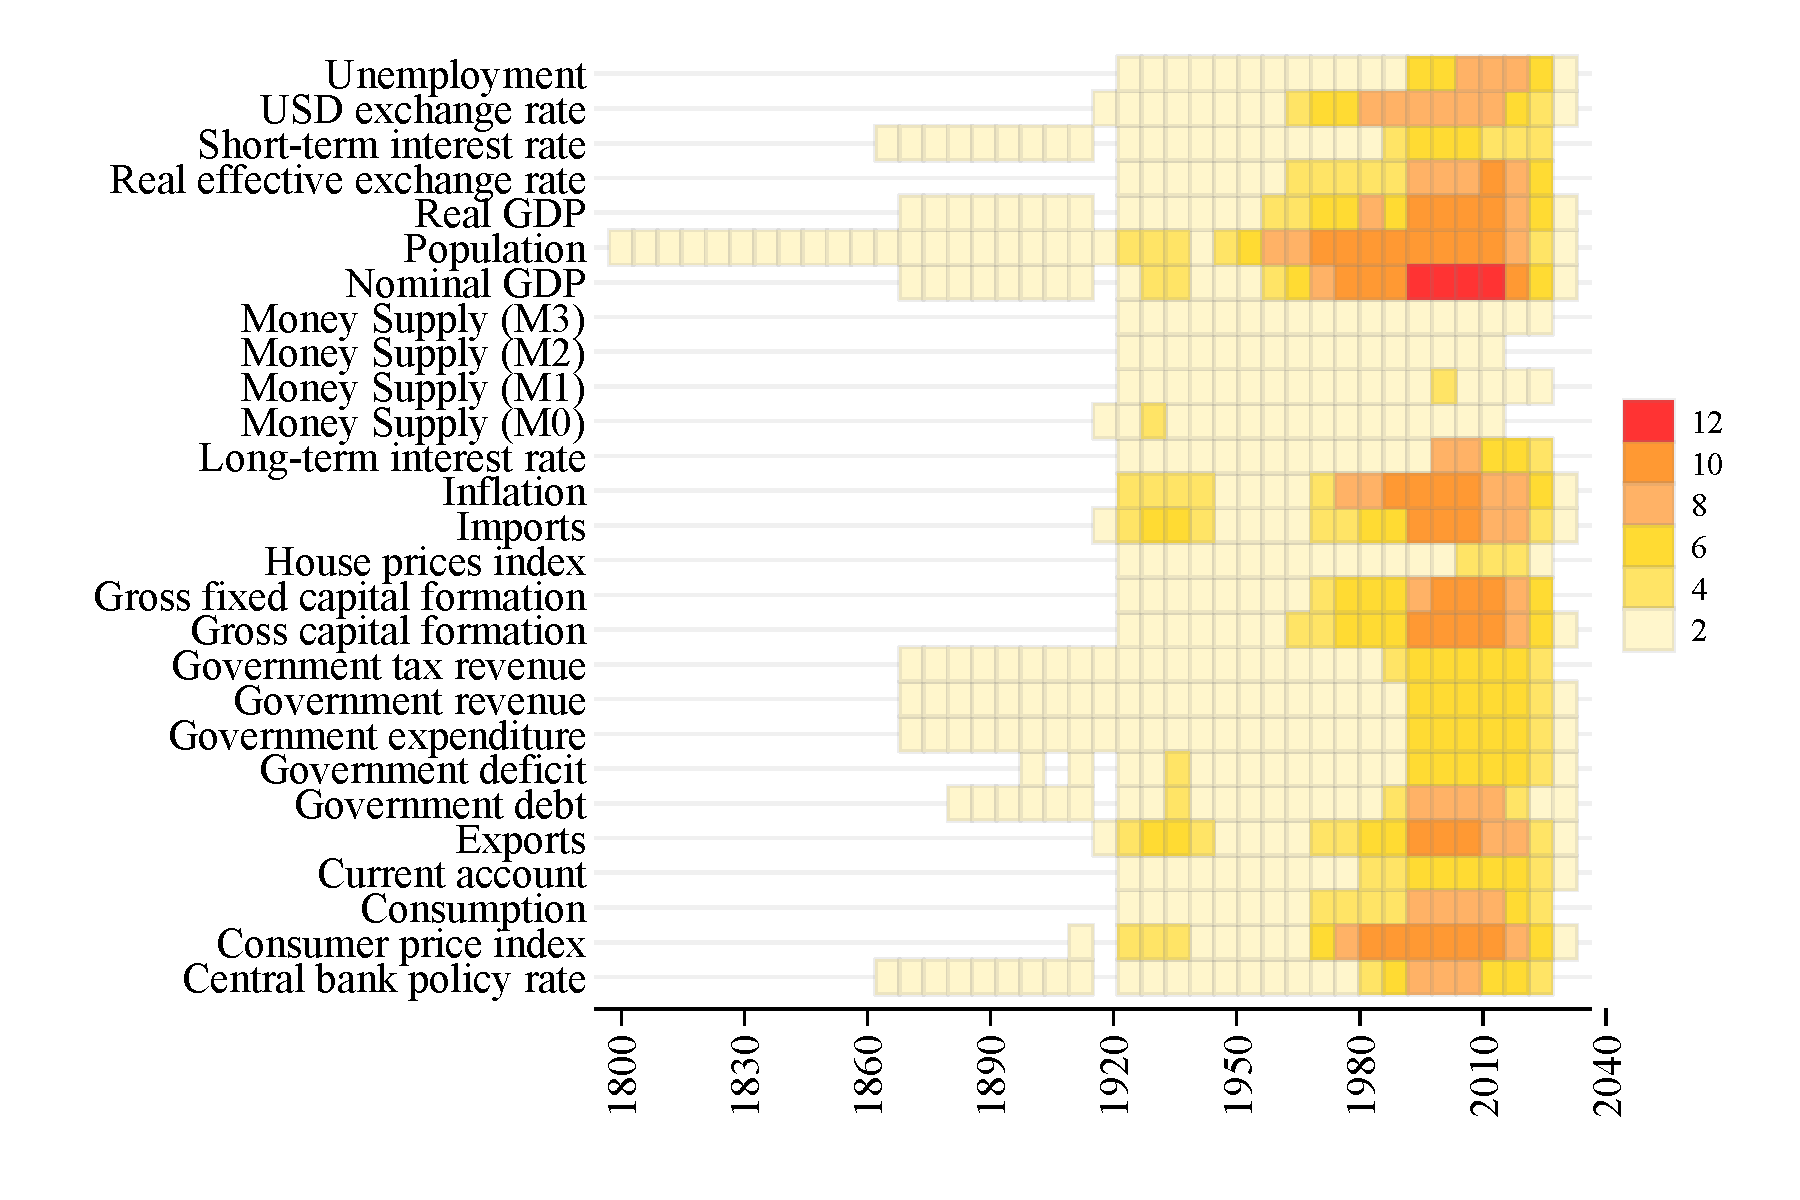
\includegraphics[width=\textwidth,height=0.8\textheight,keepaspectratio]{graphs/HUN_heatmap.pdf}
\end{figure}
\setcounter{page}{3}
\begin{adjustbox}{max totalsize={\paperwidth}{\paperheight},center}
\begin{minipage}[t][\textheight][t]{\textwidth}
\vspace*{0.5cm}
\phantomsection
\addcontentsline{toc}{section}{Current account balance}
\begin{center}
{\Large\bfseries Current account balance}
\end{center}
\vspace{0.5cm}
\begin{table}[H]
\centering
\small
\begin{tabular}{|l|l|l|}
\hline
\textbf{Source} & \textbf{Time span} & \textbf{Notes} \\
\hline
\rowcolor{white}\cite{Mitchell}& 1926 - 1979 &Spliced using overlapping data in 1980. \\
\rowcolor{lightgray}\cite{IMF_WEO}& 1980 - 1981 &Spliced using overlapping data in 1982. \\
\rowcolor{white}\cite{WDI}& 1982 - 1994 &Spliced using overlapping data in 1995. \\
\rowcolor{lightgray}\cite{OECD_EO}& 1995 - 2025 &Baseline source, overlaps with base year 2018. \\
\rowcolor{white}\cite{IMF_WEO_forecast}& 2026 - 2029 &Spliced using overlapping data in 2030. \\
\hline
\end{tabular}
\end{table}
\begin{figure}[H]
\centering
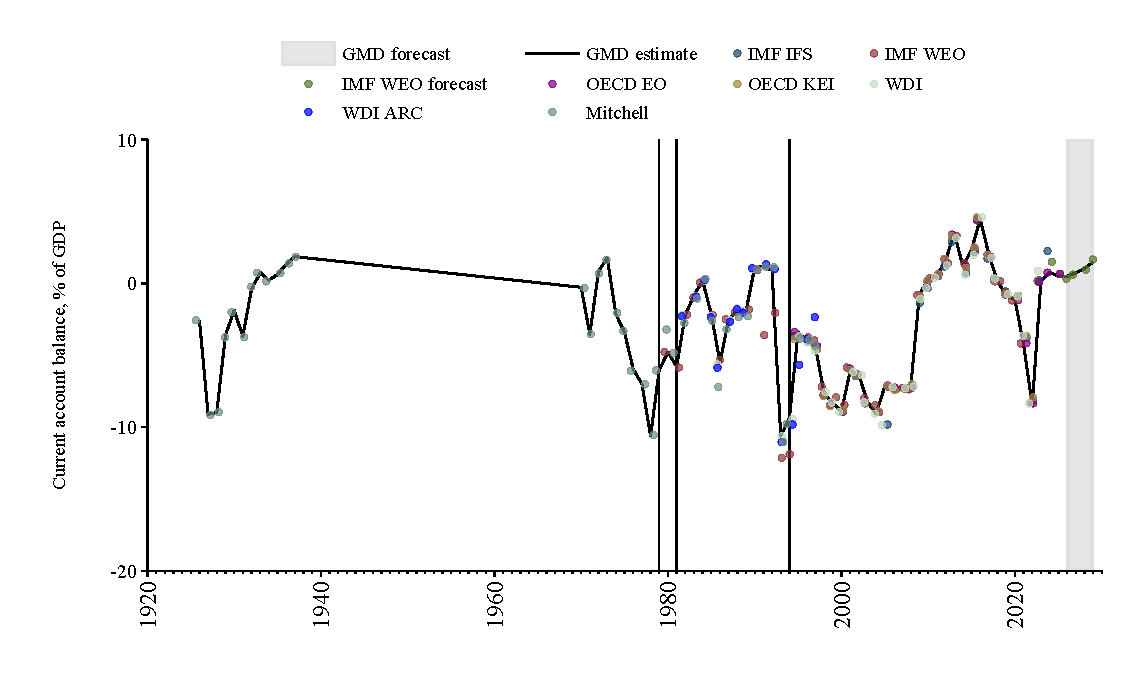
\includegraphics[width=\textwidth,height=0.6\textheight,keepaspectratio]{graphs/HUN_CA_GDP.pdf}
\end{figure}
\end{minipage}
\end{adjustbox}
\begin{adjustbox}{max totalsize={\paperwidth}{\paperheight},center}
\begin{minipage}[t][\textheight][t]{\textwidth}
\vspace*{0.5cm}
\phantomsection
\addcontentsline{toc}{section}{Consumer price index}
\begin{center}
{\Large\bfseries Consumer price index}
\end{center}
\vspace{0.5cm}
\begin{table}[H]
\centering
\small
\begin{tabular}{|l|l|l|}
\hline
\textbf{Source} & \textbf{Time span} & \textbf{Notes} \\
\hline
\rowcolor{white}\cite{HFS}& 1914 - 1924 &Spliced using overlapping data in 1925: (ratio = .3\%). \\
\rowcolor{lightgray}\cite{IHD}& 1925 - 1936 &Spliced using overlapping data in 1937: (ratio = .2\%). \\
\rowcolor{white}\cite{HFS}& 1937 - 1943 &Spliced using overlapping data in 1944: (ratio = .3\%). \\
\rowcolor{lightgray}\cite{Mitchell}& 1944 - 1969 &Spliced using overlapping data in 1970: (ratio = 38.7\%). \\
\rowcolor{white}\cite{WB_CC}& 1970 - 1971 &Spliced using overlapping data in 1972: (ratio = 2.2\%). \\
\rowcolor{lightgray}\cite{WDI}& 1972 - 1979 &Spliced using overlapping data in 1980. \\
\rowcolor{white}\cite{OECD_KEI}& 1980 - 1991 &Spliced using overlapping data in 1992: (ratio = 111.4\%). \\
\rowcolor{lightgray}\cite{BIS}& 1992 - 2024 &Baseline source, overlaps with base year 2018. \\
\rowcolor{white}\cite{AMECO}& 2025 - 2026 &Spliced using overlapping data in 2027: (ratio = 111.3\%). \\
\rowcolor{lightgray}\cite{IMF_WEO_forecast}& 2027 - 2029 &Spliced using overlapping data in 2030: (ratio = 100.1\%). \\
\hline
\end{tabular}
\end{table}
\begin{figure}[H]
\centering
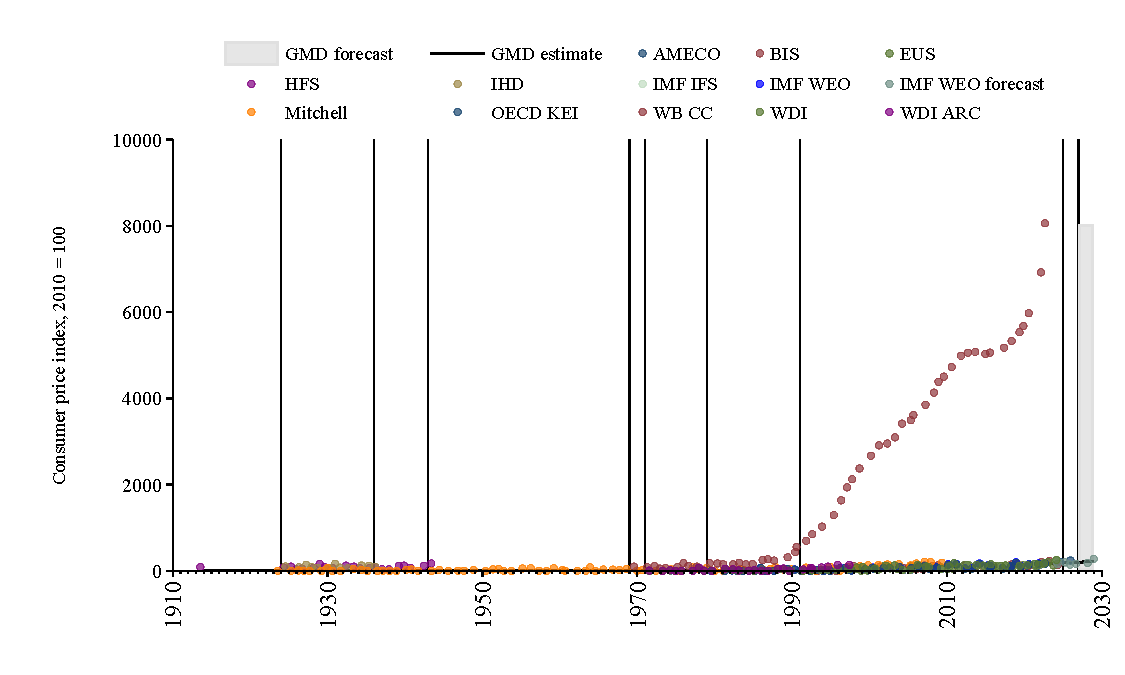
\includegraphics[width=\textwidth,height=0.6\textheight,keepaspectratio]{graphs/HUN_CPI.pdf}
\end{figure}
\end{minipage}
\end{adjustbox}
\begin{adjustbox}{max totalsize={\paperwidth}{\paperheight},center}
\begin{minipage}[t][\textheight][t]{\textwidth}
\vspace*{0.5cm}
\phantomsection
\addcontentsline{toc}{section}{House price index}
\begin{center}
{\Large\bfseries House price index}
\end{center}
\vspace{0.5cm}
\begin{table}[H]
\centering
\small
\begin{tabular}{|l|l|l|}
\hline
\textbf{Source} & \textbf{Time span} & \textbf{Notes} \\
\hline
\rowcolor{white}\cite{BIS}& 1990 - 2024 &Baseline source, overlaps with base year 2018. \\
\hline
\end{tabular}
\end{table}
\begin{figure}[H]
\centering
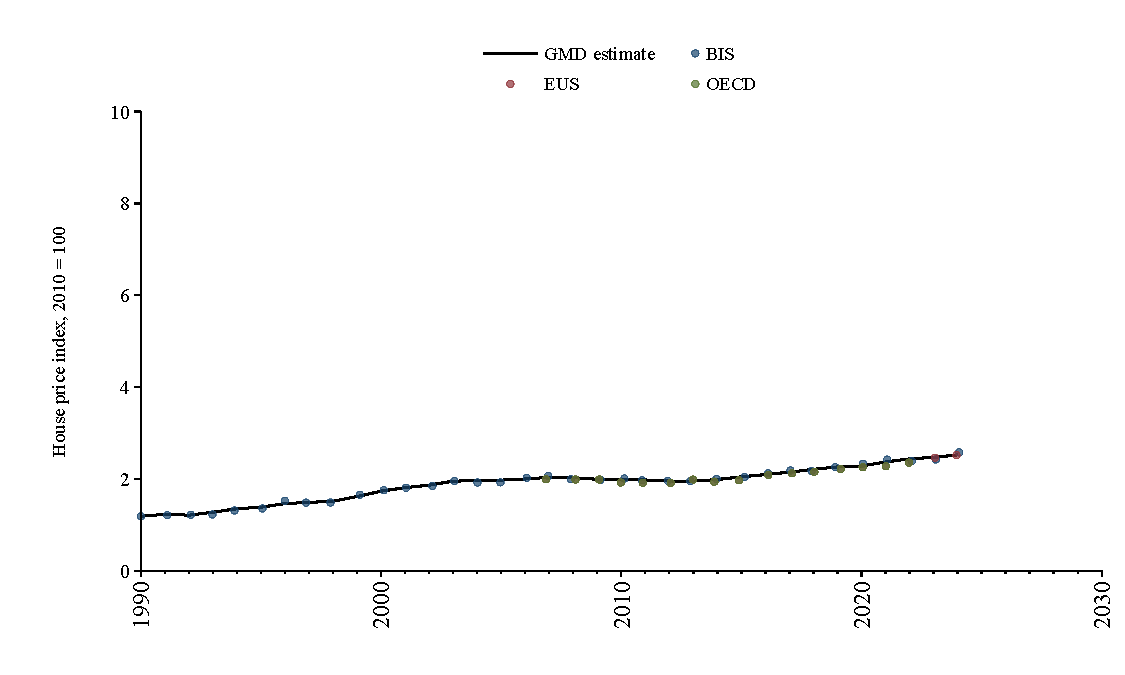
\includegraphics[width=\textwidth,height=0.6\textheight,keepaspectratio]{graphs/HUN_HPI.pdf}
\end{figure}
\end{minipage}
\end{adjustbox}
\begin{adjustbox}{max totalsize={\paperwidth}{\paperheight},center}
\begin{minipage}[t][\textheight][t]{\textwidth}
\vspace*{0.5cm}
\phantomsection
\addcontentsline{toc}{section}{Money supply (M0)}
\begin{center}
{\Large\bfseries Money supply (M0)}
\end{center}
\vspace{0.5cm}
\begin{table}[H]
\centering
\small
\begin{tabular}{|l|l|l|}
\hline
\textbf{Source} & \textbf{Time span} & \textbf{Notes} \\
\hline
\rowcolor{white}\cite{Mitchell}& 1920 - 1944 &Spliced using overlapping data in 1945. \\
\rowcolor{lightgray}\cite{IMF_MFS}& 1945 - 2008 &Spliced using overlapping data in 2009. \\
\hline
\end{tabular}
\end{table}
\begin{figure}[H]
\centering
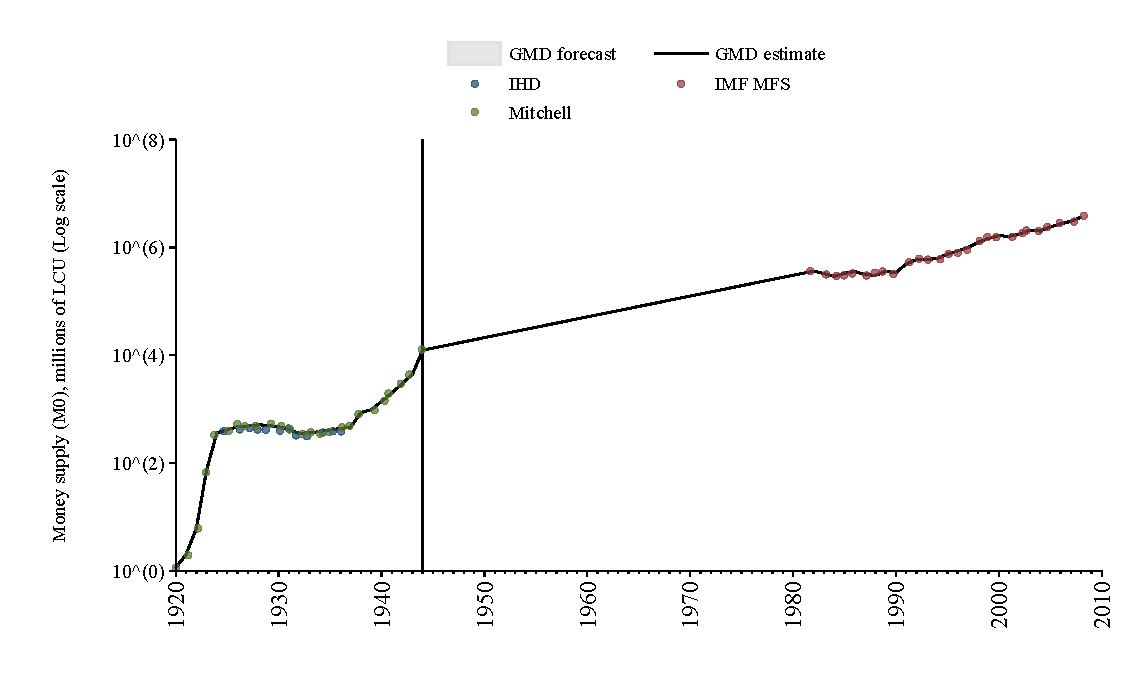
\includegraphics[width=\textwidth,height=0.6\textheight,keepaspectratio]{graphs/HUN_M0.pdf}
\end{figure}
\end{minipage}
\end{adjustbox}
\begin{adjustbox}{max totalsize={\paperwidth}{\paperheight},center}
\begin{minipage}[t][\textheight][t]{\textwidth}
\vspace*{0.5cm}
\phantomsection
\addcontentsline{toc}{section}{Money supply (M1)}
\begin{center}
{\Large\bfseries Money supply (M1)}
\end{center}
\vspace{0.5cm}
\begin{table}[H]
\centering
\small
\begin{tabular}{|l|l|l|}
\hline
\textbf{Source} & \textbf{Time span} & \textbf{Notes} \\
\hline
\rowcolor{white}\cite{IMF_MFS}& 1982 - 1993 &Spliced using overlapping data in 1994. \\
\rowcolor{lightgray}\cite{OECD_MEI}& 1994 - 2022 &Baseline source, overlaps with base year 2018. \\
\hline
\end{tabular}
\end{table}
\begin{figure}[H]
\centering
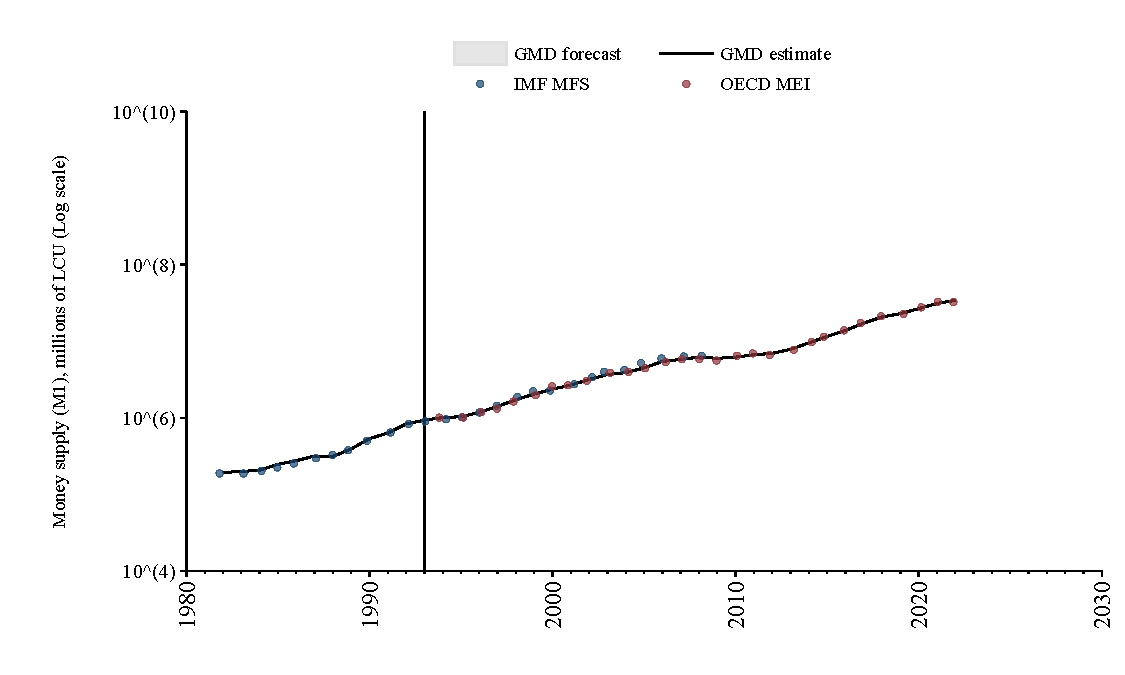
\includegraphics[width=\textwidth,height=0.6\textheight,keepaspectratio]{graphs/HUN_M1.pdf}
\end{figure}
\end{minipage}
\end{adjustbox}
\begin{adjustbox}{max totalsize={\paperwidth}{\paperheight},center}
\begin{minipage}[t][\textheight][t]{\textwidth}
\vspace*{0.5cm}
\phantomsection
\addcontentsline{toc}{section}{Money supply (M2)}
\begin{center}
{\Large\bfseries Money supply (M2)}
\end{center}
\vspace{0.5cm}
\begin{table}[H]
\centering
\small
\begin{tabular}{|l|l|l|}
\hline
\textbf{Source} & \textbf{Time span} & \textbf{Notes} \\
\hline
\rowcolor{white}\cite{IMF_MFS}& 1982 - 2008 &Spliced using overlapping data in 2009. \\
\hline
\end{tabular}
\end{table}
\begin{figure}[H]
\centering
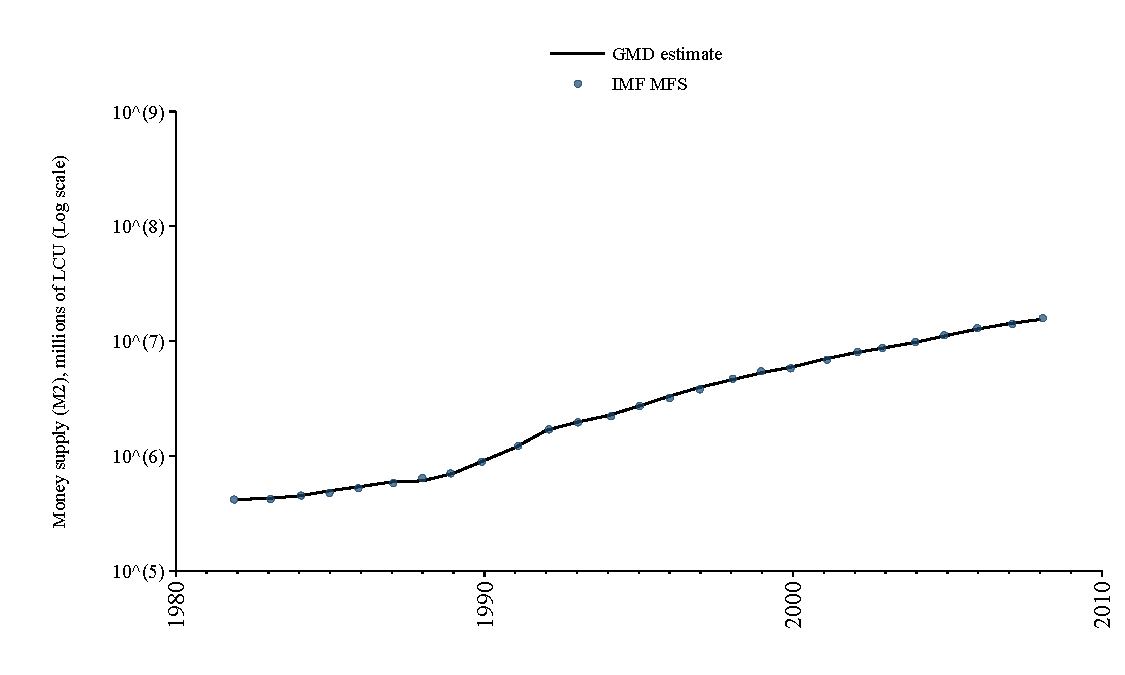
\includegraphics[width=\textwidth,height=0.6\textheight,keepaspectratio]{graphs/HUN_M2.pdf}
\end{figure}
\end{minipage}
\end{adjustbox}
\begin{adjustbox}{max totalsize={\paperwidth}{\paperheight},center}
\begin{minipage}[t][\textheight][t]{\textwidth}
\vspace*{0.5cm}
\phantomsection
\addcontentsline{toc}{section}{Money supply (M3)}
\begin{center}
{\Large\bfseries Money supply (M3)}
\end{center}
\vspace{0.5cm}
\begin{table}[H]
\centering
\small
\begin{tabular}{|l|l|l|}
\hline
\textbf{Source} & \textbf{Time span} & \textbf{Notes} \\
\hline
\rowcolor{white}\cite{OECD_MEI}& 1990 - 2022 &Baseline source, overlaps with base year 2018. \\
\hline
\end{tabular}
\end{table}
\begin{figure}[H]
\centering
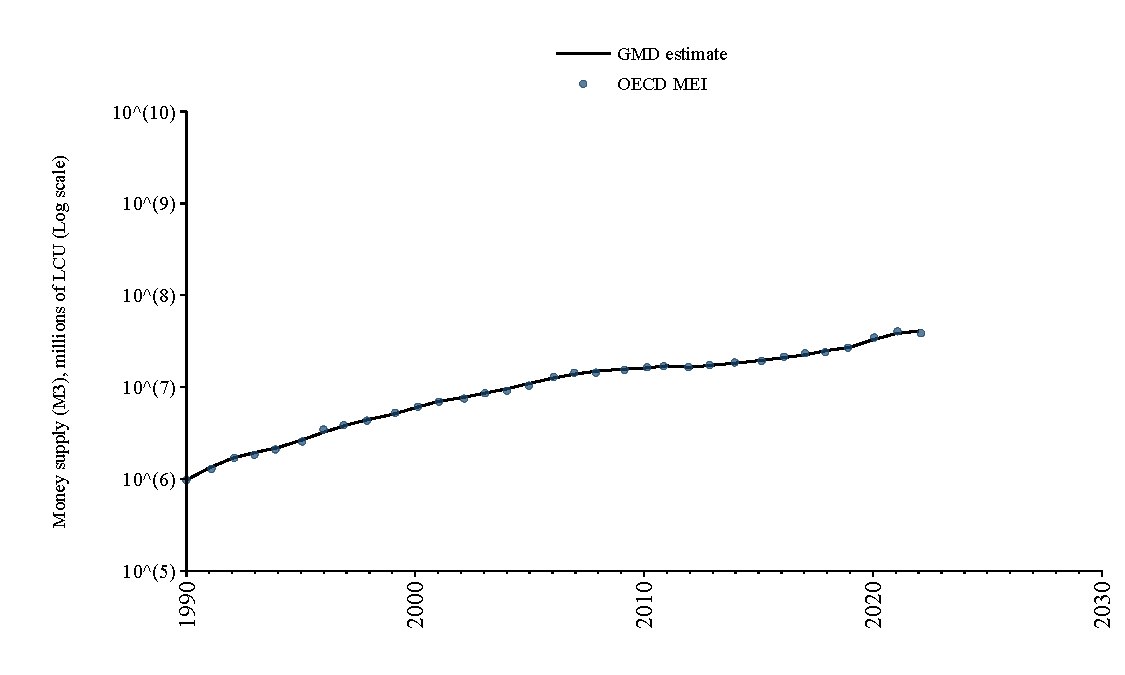
\includegraphics[width=\textwidth,height=0.6\textheight,keepaspectratio]{graphs/HUN_M3.pdf}
\end{figure}
\end{minipage}
\end{adjustbox}
\begin{adjustbox}{max totalsize={\paperwidth}{\paperheight},center}
\begin{minipage}[t][\textheight][t]{\textwidth}
\vspace*{0.5cm}
\phantomsection
\addcontentsline{toc}{section}{Real effective exchange rate}
\begin{center}
{\Large\bfseries Real effective exchange rate}
\end{center}
\vspace{0.5cm}
\begin{table}[H]
\centering
\small
\begin{tabular}{|l|l|l|}
\hline
\textbf{Source} & \textbf{Time span} & \textbf{Notes} \\
\hline
\rowcolor{white}\cite{LUND}& 1927 - 1959 &Spliced using overlapping data in 1960: (ratio = 67\%). \\
\rowcolor{lightgray}\cite{BRUEGEL}& 1960 - 1979 &Spliced using overlapping data in 1980: (ratio = 105.5\%). \\
\rowcolor{white}\cite{WDI_ARC}& 1980 - 1990 &Spliced using overlapping data in 1991: (ratio = 52.7\%). \\
\rowcolor{lightgray}\cite{WDI}& 1991 - 2023 &Baseline source, overlaps with base year 2018. \\
\rowcolor{white}\cite{BIS}& 2024 - 2025 &Spliced using overlapping data in 2026: (ratio = 86\%). \\
\hline
\end{tabular}
\end{table}
\begin{figure}[H]
\centering
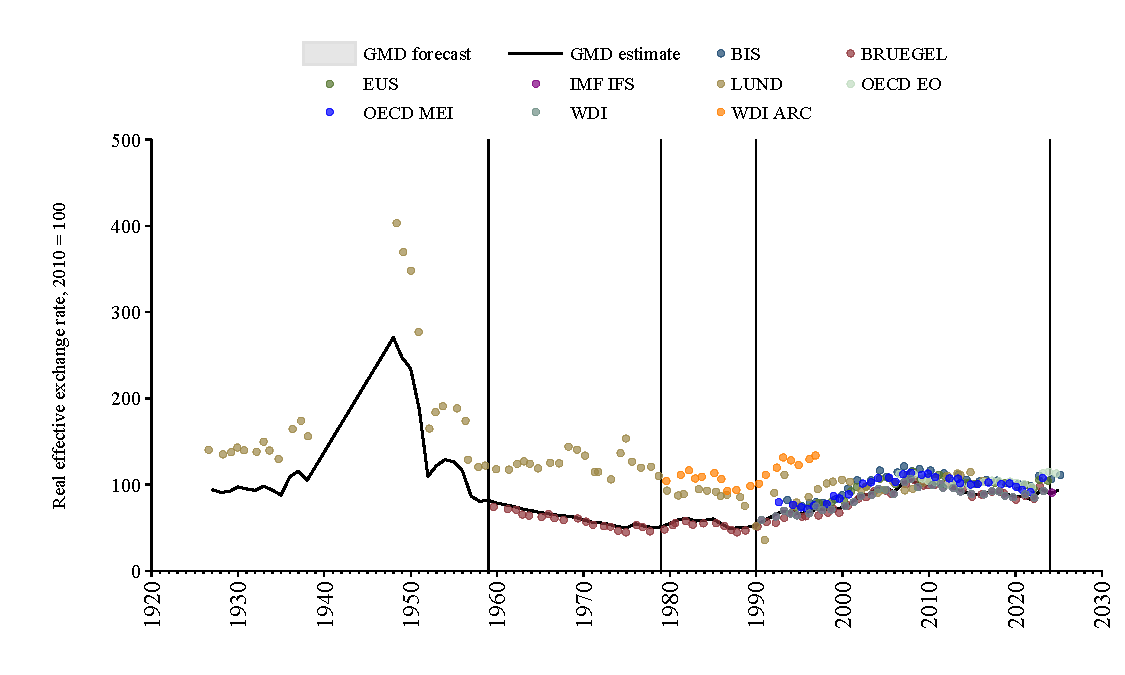
\includegraphics[width=\textwidth,height=0.6\textheight,keepaspectratio]{graphs/HUN_REER.pdf}
\end{figure}
\end{minipage}
\end{adjustbox}
\begin{adjustbox}{max totalsize={\paperwidth}{\paperheight},center}
\begin{minipage}[t][\textheight][t]{\textwidth}
\vspace*{0.5cm}
\phantomsection
\addcontentsline{toc}{section}{USD exchange rate}
\begin{center}
{\Large\bfseries USD exchange rate}
\end{center}
\vspace{0.5cm}
\begin{table}[H]
\centering
\small
\begin{tabular}{|l|l|l|}
\hline
\textbf{Source} & \textbf{Time span} & \textbf{Notes} \\
\hline
\rowcolor{white}\cite{Tena}& 1920 - 1938 &Spliced using overlapping data in 1939. \\
\rowcolor{lightgray}\cite{BIS}& 1939 - 2024 &Baseline source, overlaps with base year 2018. \\
\rowcolor{white}\cite{OECD_EO}& 2025 - 2025 &Spliced using overlapping data in 2026. \\
\hline
\end{tabular}
\end{table}
\begin{figure}[H]
\centering
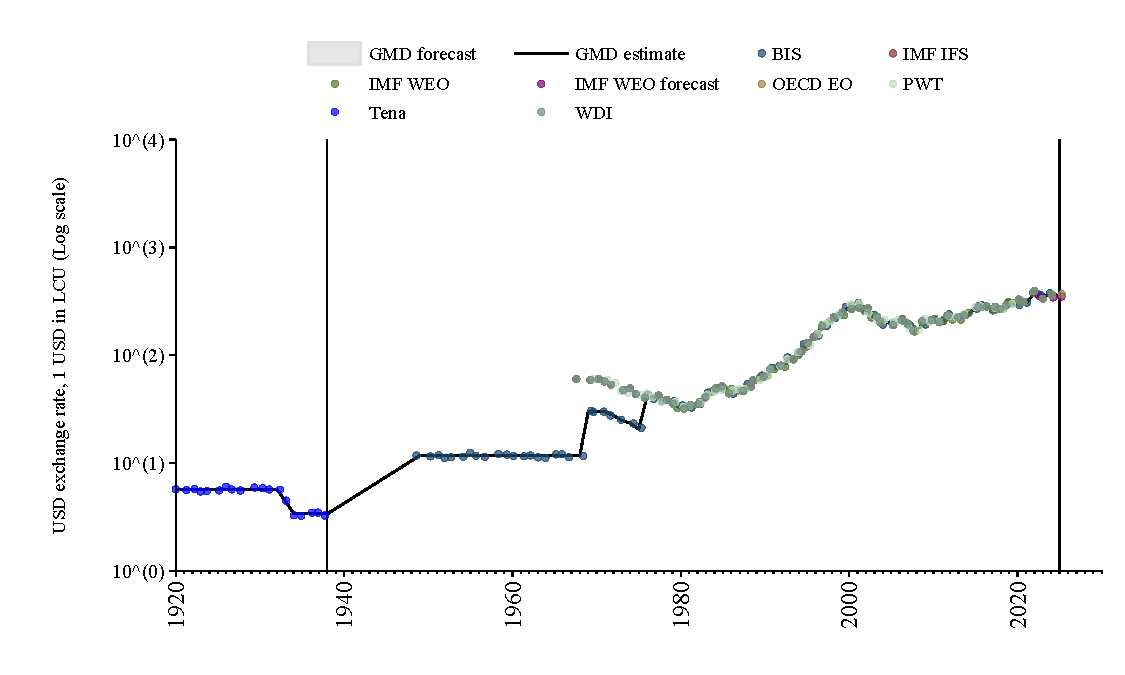
\includegraphics[width=\textwidth,height=0.6\textheight,keepaspectratio]{graphs/HUN_USDfx.pdf}
\end{figure}
\end{minipage}
\end{adjustbox}
\begin{adjustbox}{max totalsize={\paperwidth}{\paperheight},center}
\begin{minipage}[t][\textheight][t]{\textwidth}
\vspace*{0.5cm}
\phantomsection
\addcontentsline{toc}{section}{Central bank policy rate}
\begin{center}
{\Large\bfseries Central bank policy rate}
\end{center}
\vspace{0.5cm}
\begin{table}[H]
\centering
\small
\begin{tabular}{|l|l|l|}
\hline
\textbf{Source} & \textbf{Time span} & \textbf{Notes} \\
\hline
\rowcolor{white}\cite{NBS}& 1863 - 1913 &Spliced using overlapping data in 1914. \\
\rowcolor{lightgray}\cite{OECD_MEI}& 1914 - 1984 &Spliced using overlapping data in 1985. \\
\rowcolor{white}\cite{IMF_MFS}& 1985 - 1986 &Spliced using overlapping data in 1987. \\
\rowcolor{lightgray}\cite{BIS}& 1987 - 2025 &Baseline source, overlaps with base year 2018. \\
\hline
\end{tabular}
\end{table}
\begin{figure}[H]
\centering
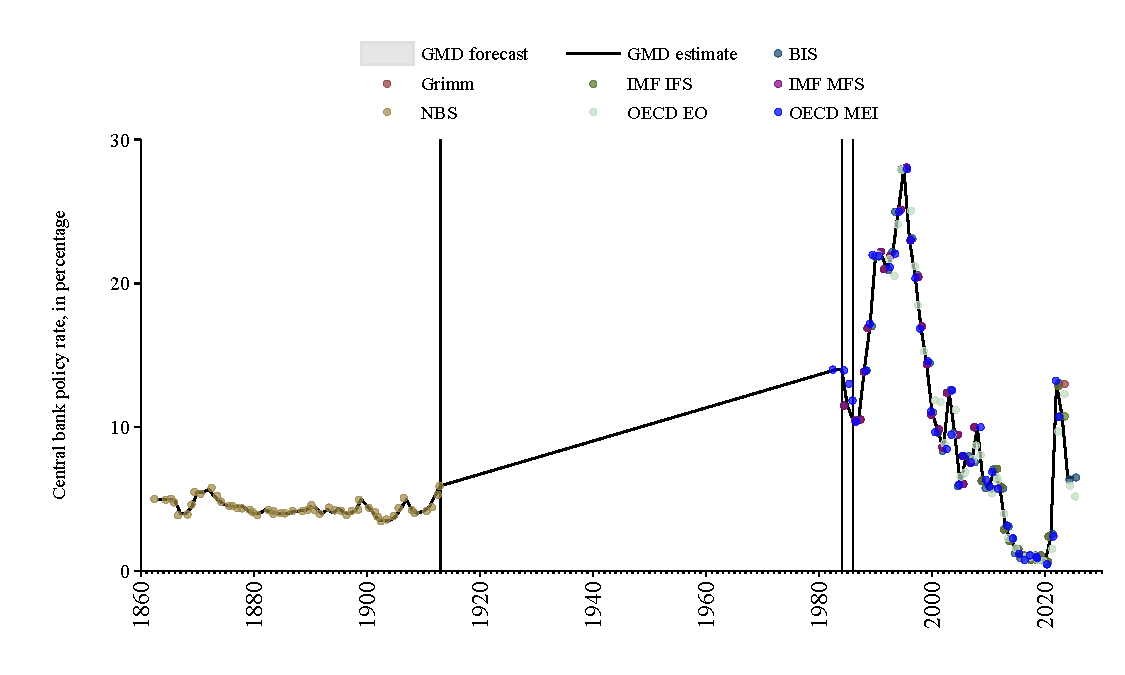
\includegraphics[width=\textwidth,height=0.6\textheight,keepaspectratio]{graphs/HUN_cbrate.pdf}
\end{figure}
\end{minipage}
\end{adjustbox}
\begin{adjustbox}{max totalsize={\paperwidth}{\paperheight},center}
\begin{minipage}[t][\textheight][t]{\textwidth}
\vspace*{0.5cm}
\phantomsection
\addcontentsline{toc}{section}{Total consumption}
\begin{center}
{\Large\bfseries Total consumption}
\end{center}
\vspace{0.5cm}
\begin{table}[H]
\centering
\small
\begin{tabular}{|l|l|l|}
\hline
\textbf{Source} & \textbf{Time span} & \textbf{Notes} \\
\hline
\rowcolor{white}\cite{WDI_ARC}& 1960 - 1969 &Spliced using overlapping data in 1970: (ratio = 103.1\%). \\
\rowcolor{lightgray}\cite{AMECO}& 1970 - 1990 &Spliced using overlapping data in 1991: (ratio = 100.1\%). \\
\rowcolor{white}\cite{OECD_EO}& 1991 - 2025 &Baseline source, overlaps with base year 2018. \\
\rowcolor{lightgray}\cite{AMECO}& 2026 - 2026 &Spliced using overlapping data in 2027: (ratio = 97.6\%). \\
\hline
\end{tabular}
\end{table}
\begin{figure}[H]
\centering
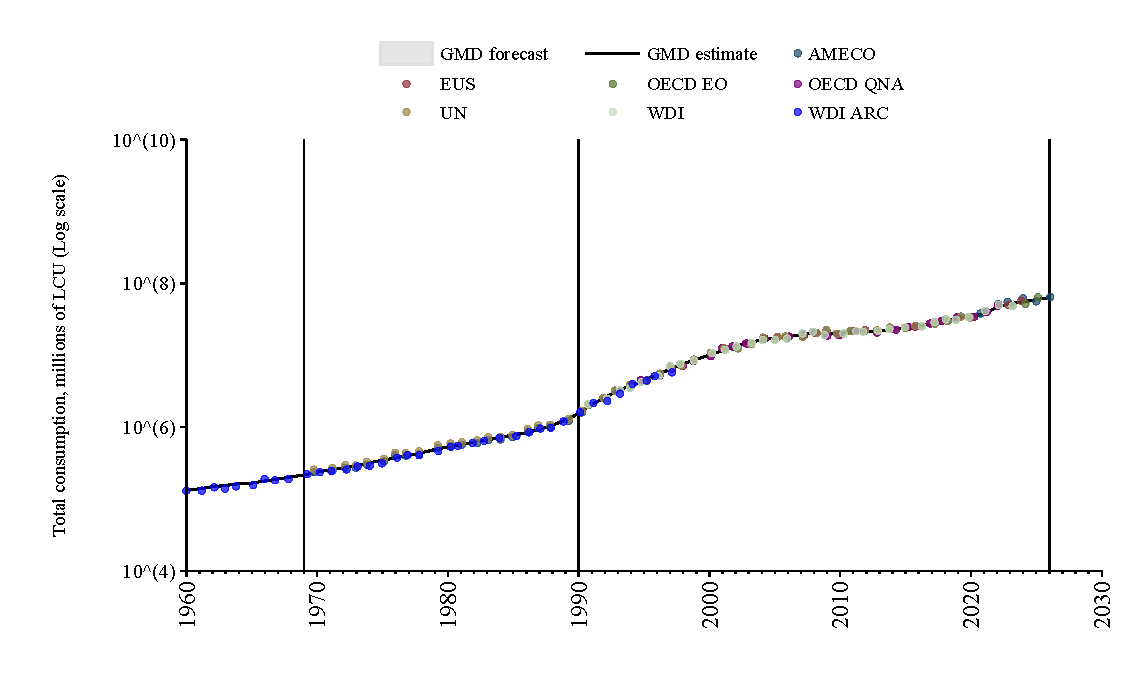
\includegraphics[width=\textwidth,height=0.6\textheight,keepaspectratio]{graphs/HUN_cons.pdf}
\end{figure}
\end{minipage}
\end{adjustbox}
\begin{adjustbox}{max totalsize={\paperwidth}{\paperheight},center}
\begin{minipage}[t][\textheight][t]{\textwidth}
\vspace*{0.5cm}
\phantomsection
\addcontentsline{toc}{section}{Total consumption to GDP ratio}
\begin{center}
{\Large\bfseries Total consumption to GDP ratio}
\end{center}
\vspace{0.5cm}
\begin{table}[H]
\centering
\small
\begin{tabular}{|l|l|l|}
\hline
\textbf{Source} & \textbf{Time span} & \textbf{Notes} \\
\hline
\rowcolor{white}\cite{WDI_ARC}& 1960 - 1990 &Spliced using overlapping data in 1991: (ratio = 99.2\%). \\
\rowcolor{lightgray}\cite{WDI}& 1991 - 2023 &Baseline source, overlaps with base year 2018. \\
\rowcolor{white}\cite{EUS}& 2024 - 2024 &Spliced using overlapping data in 2025. \\
\rowcolor{lightgray}\cite{OECD_EO}& 2025 - 2025 &Spliced using overlapping data in 2026: (ratio = 104.3\%). \\
\rowcolor{white}\cite{AMECO}& 2026 - 2026 &Spliced using overlapping data in 2027: (ratio = 99.9\%). \\
\hline
\end{tabular}
\end{table}
\begin{figure}[H]
\centering
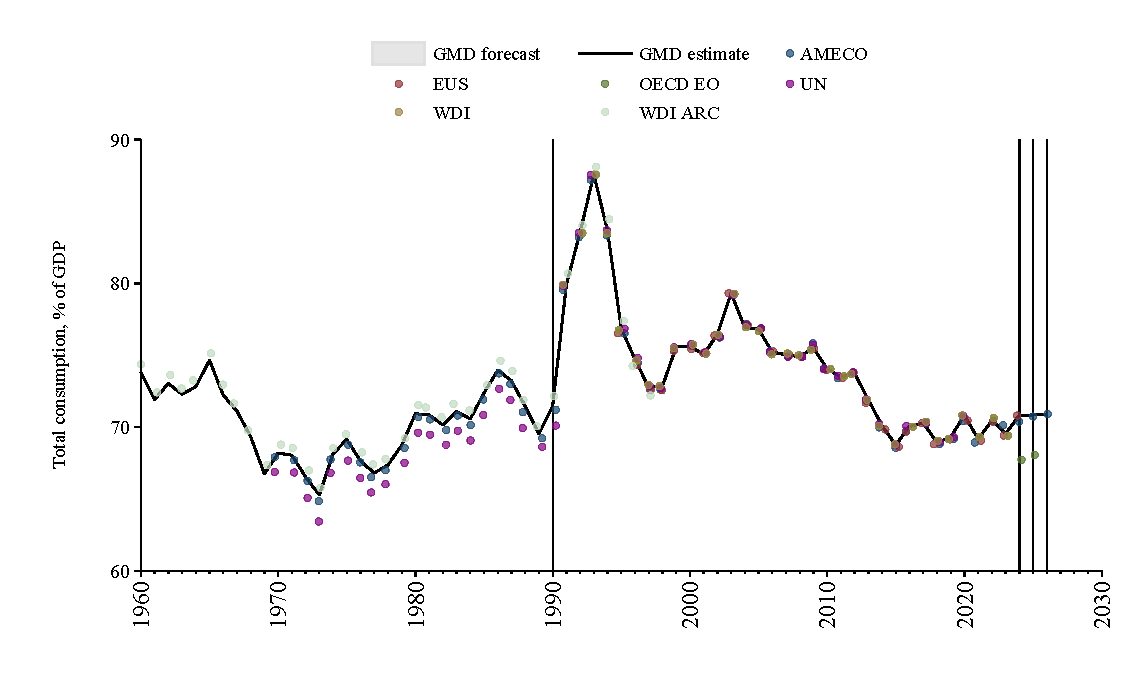
\includegraphics[width=\textwidth,height=0.6\textheight,keepaspectratio]{graphs/HUN_cons_GDP.pdf}
\end{figure}
\end{minipage}
\end{adjustbox}
\begin{adjustbox}{max totalsize={\paperwidth}{\paperheight},center}
\begin{minipage}[t][\textheight][t]{\textwidth}
\vspace*{0.5cm}
\phantomsection
\addcontentsline{toc}{section}{Exports}
\begin{center}
{\Large\bfseries Exports}
\end{center}
\vspace{0.5cm}
\begin{table}[H]
\centering
\small
\begin{tabular}{|l|l|l|}
\hline
\textbf{Source} & \textbf{Time span} & \textbf{Notes} \\
\hline
\rowcolor{white}\cite{Tena}& 1920 - 1938 &Spliced using overlapping data in 1939: (ratio = 339.2\%). \\
\rowcolor{lightgray}\cite{Mitchell}& 1939 - 1969 &Spliced using overlapping data in 1970: (ratio = 339.5\%). \\
\rowcolor{white}\cite{UN}& 1970 - 1977 &Spliced using overlapping data in 1978: (ratio = 102\%). \\
\rowcolor{lightgray}\cite{AMECO}& 1978 - 1990 &Spliced using overlapping data in 1991: (ratio = 99.9\%). \\
\rowcolor{white}\cite{OECD_EO}& 1991 - 2025 &Baseline source, overlaps with base year 2018. \\
\rowcolor{lightgray}\cite{AMECO}& 2026 - 2026 &Spliced using overlapping data in 2027: (ratio = 102.3\%). \\
\rowcolor{white}\cite{IMF_WEO_forecast}& 2027 - 2029 &Spliced using overlapping data in 2030: (ratio = 104.6\%). \\
\hline
\end{tabular}
\end{table}
\begin{figure}[H]
\centering
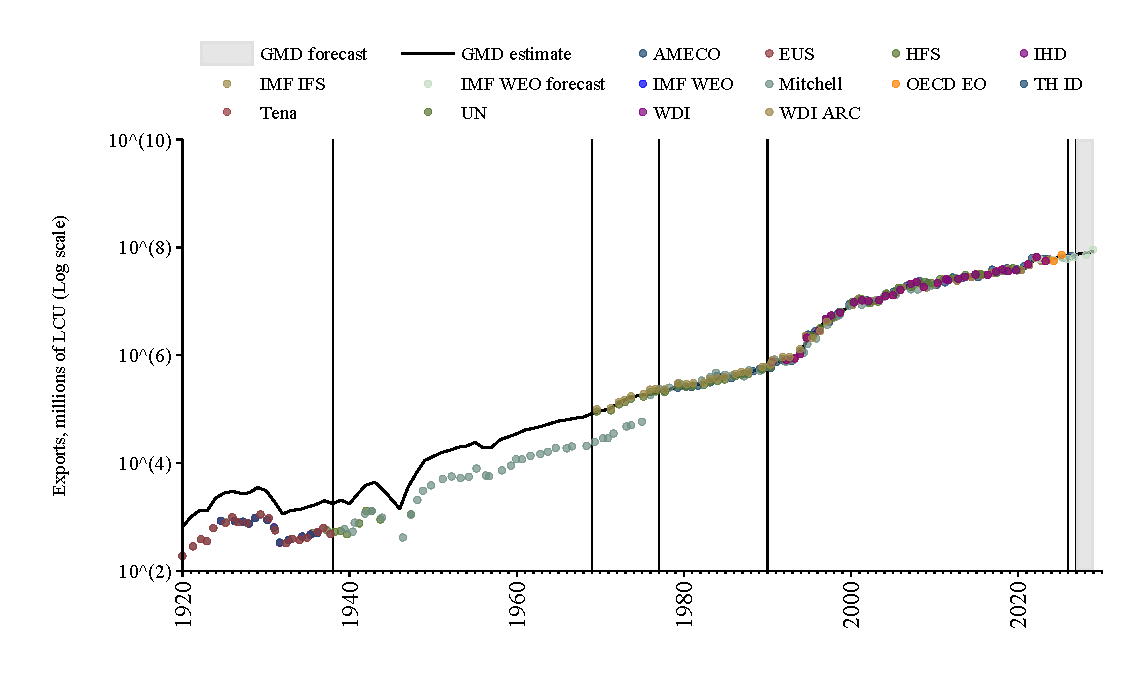
\includegraphics[width=\textwidth,height=0.6\textheight,keepaspectratio]{graphs/HUN_exports.pdf}
\end{figure}
\end{minipage}
\end{adjustbox}
\begin{adjustbox}{max totalsize={\paperwidth}{\paperheight},center}
\begin{minipage}[t][\textheight][t]{\textwidth}
\vspace*{0.5cm}
\phantomsection
\addcontentsline{toc}{section}{Exports to GDP ratio}
\begin{center}
{\Large\bfseries Exports to GDP ratio}
\end{center}
\vspace{0.5cm}
\begin{table}[H]
\centering
\small
\begin{tabular}{|l|l|l|}
\hline
\textbf{Source} & \textbf{Time span} & \textbf{Notes} \\
\hline
\rowcolor{white}\cite{Mitchell}& 1921 - 1969 &Spliced using overlapping data in 1970: (ratio = 236.1\%). \\
\rowcolor{lightgray}\cite{UN}& 1970 - 1990 &Spliced using overlapping data in 1991. \\
\rowcolor{white}\cite{OECD_EO}& 1991 - 2025 &Baseline source, overlaps with base year 2018. \\
\rowcolor{lightgray}\cite{AMECO}& 2026 - 2026 &Spliced using overlapping data in 2027: (ratio = 100.3\%). \\
\rowcolor{white}\cite{IMF_WEO_forecast}& 2027 - 2029 &Spliced using overlapping data in 2030: (ratio = 101.5\%). \\
\hline
\end{tabular}
\end{table}
\begin{figure}[H]
\centering
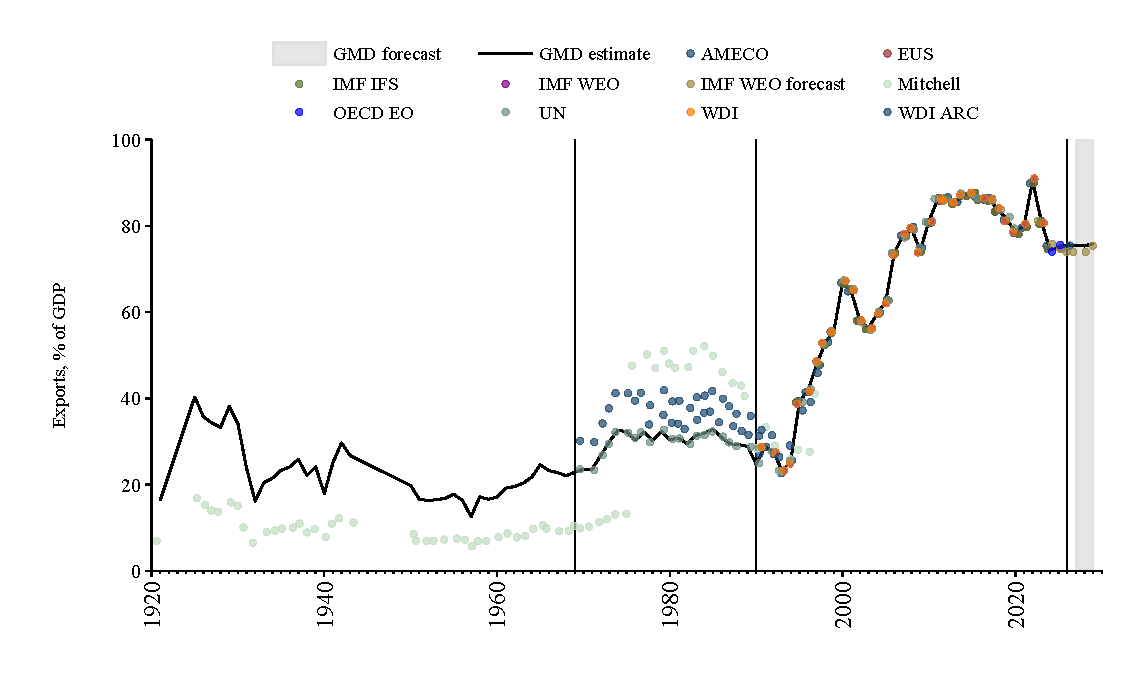
\includegraphics[width=\textwidth,height=0.6\textheight,keepaspectratio]{graphs/HUN_exports_GDP.pdf}
\end{figure}
\end{minipage}
\end{adjustbox}
\begin{adjustbox}{max totalsize={\paperwidth}{\paperheight},center}
\begin{minipage}[t][\textheight][t]{\textwidth}
\vspace*{0.5cm}
\phantomsection
\addcontentsline{toc}{section}{Fixed investment}
\begin{center}
{\Large\bfseries Fixed investment}
\end{center}
\vspace{0.5cm}
\begin{table}[H]
\centering
\small
\begin{tabular}{|l|l|l|}
\hline
\textbf{Source} & \textbf{Time span} & \textbf{Notes} \\
\hline
\rowcolor{white}\cite{WDI_ARC}& 1960 - 1969 &Spliced using overlapping data in 1970: (ratio = 127.4\%). \\
\rowcolor{lightgray}\cite{AMECO}& 1970 - 1990 &Spliced using overlapping data in 1991. \\
\rowcolor{white}\cite{OECD_EO}& 1991 - 2025 &Baseline source, overlaps with base year 2018. \\
\rowcolor{lightgray}\cite{AMECO}& 2026 - 2026 &Spliced using overlapping data in 2027: (ratio = 110.4\%). \\
\hline
\end{tabular}
\end{table}
\begin{figure}[H]
\centering
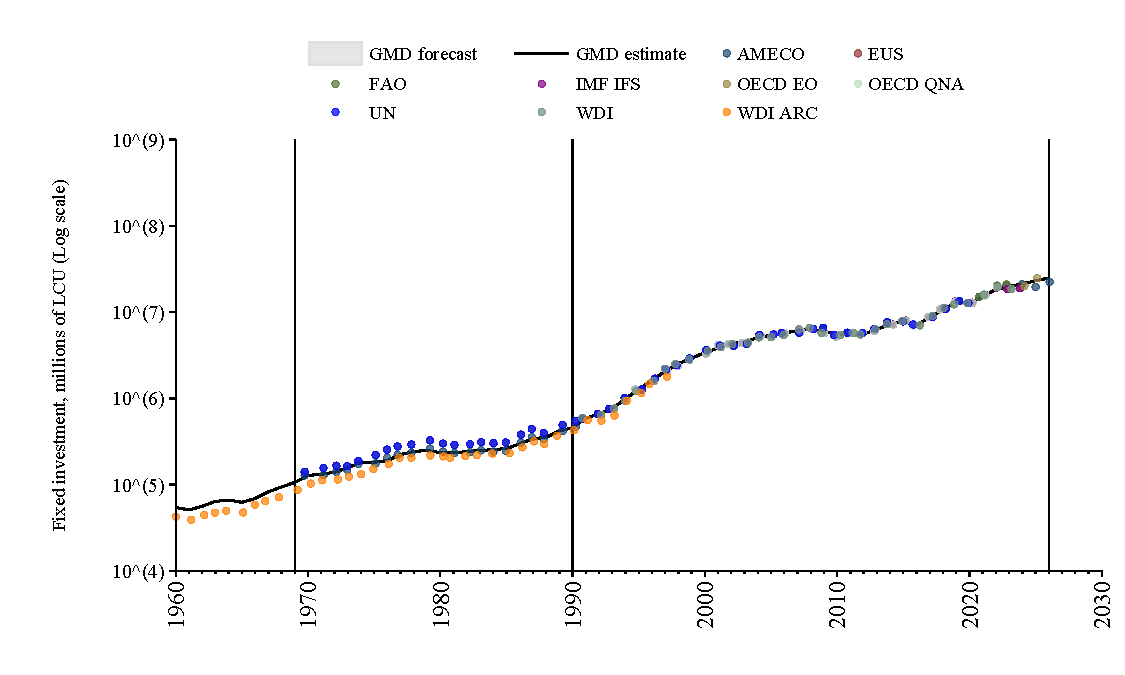
\includegraphics[width=\textwidth,height=0.6\textheight,keepaspectratio]{graphs/HUN_finv.pdf}
\end{figure}
\end{minipage}
\end{adjustbox}
\begin{adjustbox}{max totalsize={\paperwidth}{\paperheight},center}
\begin{minipage}[t][\textheight][t]{\textwidth}
\vspace*{0.5cm}
\phantomsection
\addcontentsline{toc}{section}{Fixed investment to GDP ratio}
\begin{center}
{\Large\bfseries Fixed investment to GDP ratio}
\end{center}
\vspace{0.5cm}
\begin{table}[H]
\centering
\small
\begin{tabular}{|l|l|l|}
\hline
\textbf{Source} & \textbf{Time span} & \textbf{Notes} \\
\hline
\rowcolor{white}\cite{WDI_ARC}& 1960 - 1969 &Spliced using overlapping data in 1970: (ratio = 121.8\%). \\
\rowcolor{lightgray}\cite{UN}& 1970 - 1990 &Spliced using overlapping data in 1991: (ratio = 99.7\%). \\
\rowcolor{white}\cite{WDI}& 1991 - 1994 &Spliced using overlapping data in 1995: (ratio = 99.7\%). \\
\rowcolor{lightgray}\cite{EUS}& 1995 - 2024 &Baseline source, overlaps with base year 2018. \\
\rowcolor{white}\cite{OECD_EO}& 2025 - 2025 &Spliced using overlapping data in 2026: (ratio = 89.9\%). \\
\rowcolor{lightgray}\cite{AMECO}& 2026 - 2026 &Spliced using overlapping data in 2027: (ratio = 97.3\%). \\
\hline
\end{tabular}
\end{table}
\begin{figure}[H]
\centering
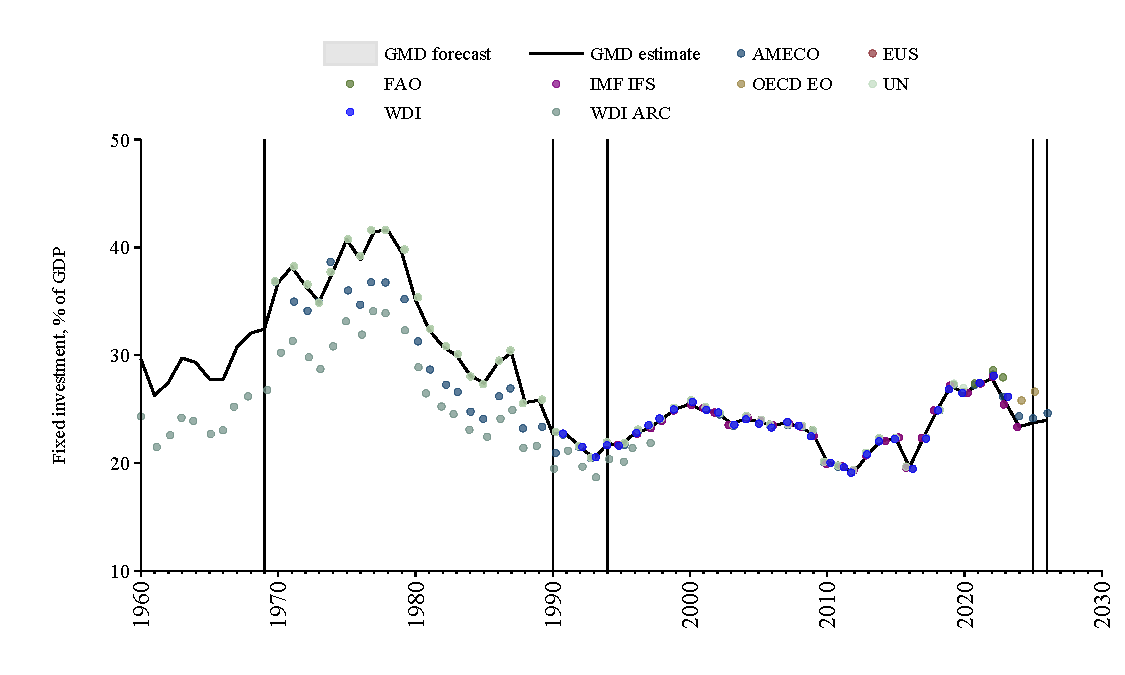
\includegraphics[width=\textwidth,height=0.6\textheight,keepaspectratio]{graphs/HUN_finv_GDP.pdf}
\end{figure}
\end{minipage}
\end{adjustbox}
\begin{adjustbox}{max totalsize={\paperwidth}{\paperheight},center}
\begin{minipage}[t][\textheight][t]{\textwidth}
\vspace*{0.5cm}
\phantomsection
\addcontentsline{toc}{section}{Government debt}
\begin{center}
{\Large\bfseries Government debt}
\end{center}
\vspace{0.5cm}
\begin{table}[H]
\centering
\small
\begin{tabular}{|l|l|l|}
\hline
\textbf{Source} & \textbf{Time span} & \textbf{Notes} \\
\hline
\rowcolor{white}\cite{RR_debt}& 1880 - 1913 &Spliced using overlapping data in 1914. \\
\rowcolor{lightgray}\cite{IMF_FPP}& 1914 - 1943 &Spliced using overlapping data in 1944. Data refers to general government.\\
\rowcolor{white}\cite{WDI_ARC}& 1944 - 1981 &Spliced using overlapping data in 1982. Data refers to central government.\\
\rowcolor{lightgray}\cite{IMF_HDD}& 1982 - 1988 &Spliced using overlapping data in 1989. Data refers to general government.\\
\rowcolor{white}\cite{IMF_GDD}& 1989 - 2018 &Spliced using overlapping data in 2019. Data refers to central government.\\
\rowcolor{lightgray}\cite{IMF_FPP}& 2019 - 2023 &Spliced using overlapping data in 2024. Data refers to general government.\\
\rowcolor{white}\cite{OECD_EO}& 2024 - 2025 &Spliced using overlapping data in 2026. Data refers to general government.\\
\rowcolor{lightgray}\cite{IMF_WEO_forecast}& 2026 - 2029 &Spliced using overlapping data in 2030. \\
\hline
\end{tabular}
\end{table}
\begin{figure}[H]
\centering
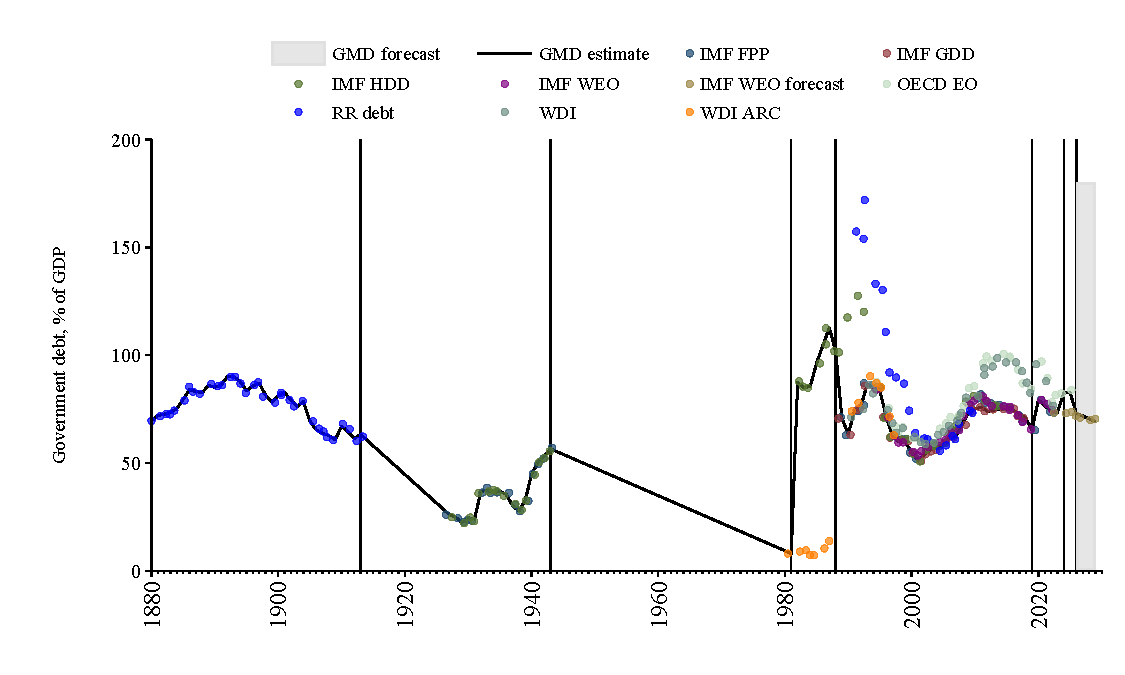
\includegraphics[width=\textwidth,height=0.6\textheight,keepaspectratio]{graphs/HUN_govdebt_GDP.pdf}
\end{figure}
\end{minipage}
\end{adjustbox}
\begin{adjustbox}{max totalsize={\paperwidth}{\paperheight},center}
\begin{minipage}[t][\textheight][t]{\textwidth}
\vspace*{0.5cm}
\phantomsection
\addcontentsline{toc}{section}{Government deficit}
\begin{center}
{\Large\bfseries Government deficit}
\end{center}
\vspace{0.5cm}
\begin{table}[H]
\centering
\small
\begin{tabular}{|l|l|l|}
\hline
\textbf{Source} & \textbf{Time span} & \textbf{Notes} \\
\hline
\rowcolor{white}\cite{Mitchell}& 1900 - 1927 &Spliced using overlapping data in 1928. \\
\rowcolor{lightgray}\cite{IMF_FPP}& 1928 - 1941 &Spliced using overlapping data in 1942. \\
\rowcolor{white}\cite{IMF_GFS}& 1942 - 1994 &Spliced using overlapping data in 1995. \\
\rowcolor{lightgray}\cite{EUS}& 1995 - 2024 &Baseline source, overlaps with base year 2018. \\
\rowcolor{white}\cite{IMF_WEO_forecast}& 2025 - 2029 &Spliced using overlapping data in 2030. \\
\hline
\end{tabular}
\end{table}
\begin{figure}[H]
\centering
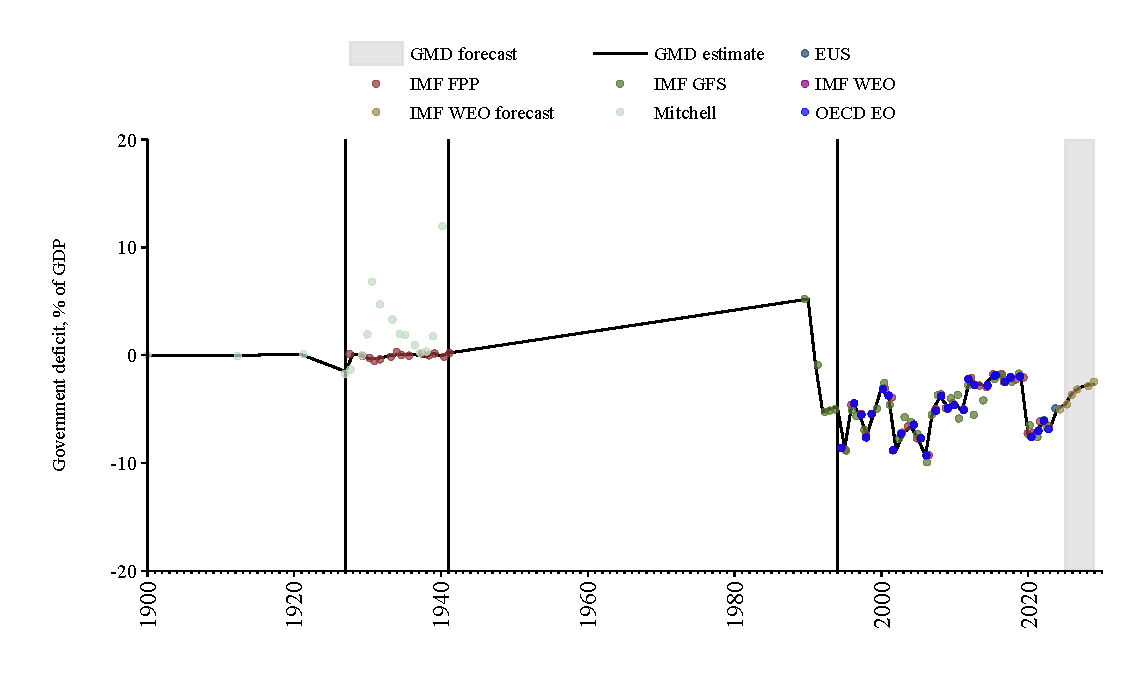
\includegraphics[width=\textwidth,height=0.6\textheight,keepaspectratio]{graphs/HUN_govdef_GDP.pdf}
\end{figure}
\end{minipage}
\end{adjustbox}
\begin{adjustbox}{max totalsize={\paperwidth}{\paperheight},center}
\begin{minipage}[t][\textheight][t]{\textwidth}
\vspace*{0.5cm}
\phantomsection
\addcontentsline{toc}{section}{Government expenditure}
\begin{center}
{\Large\bfseries Government expenditure}
\end{center}
\vspace{0.5cm}
\begin{table}[H]
\centering
\small
\begin{tabular}{|l|l|l|}
\hline
\textbf{Source} & \textbf{Time span} & \textbf{Notes} \\
\hline
\rowcolor{white}\cite{Mitchell}& 1868 - 1899 &Spliced using overlapping data in 1900: (ratio = 128.3\%). \\
\rowcolor{lightgray}\cite{GMD_estimated}& 1900 - 1900 &Spliced using overlapping data in 1901: (ratio = 21.7\%). \\
\rowcolor{white}\cite{Mitchell}& 1901 - 1911 &Spliced using overlapping data in 1912: (ratio = 128.3\%). \\
\rowcolor{lightgray}\cite{GMD_estimated}& 1912 - 1912 &Spliced using overlapping data in 1913: (ratio = 23.6\%). \\
\rowcolor{white}\cite{Mitchell}& 1913 - 1920 &Spliced using overlapping data in 1921: (ratio = 128.3\%). \\
\rowcolor{lightgray}\cite{GMD_estimated}& 1921 - 1921 &Spliced using overlapping data in 1922. \\
\rowcolor{white}\cite{Mitchell}& 1922 - 1924 &Spliced using overlapping data in 1925: (ratio = 128.3\%). \\
\rowcolor{lightgray}\cite{GMD_estimated}& 1925 - 2029 &Baseline source, overlaps with base year 2018. \\
\hline
\end{tabular}
\end{table}
\begin{figure}[H]
\centering
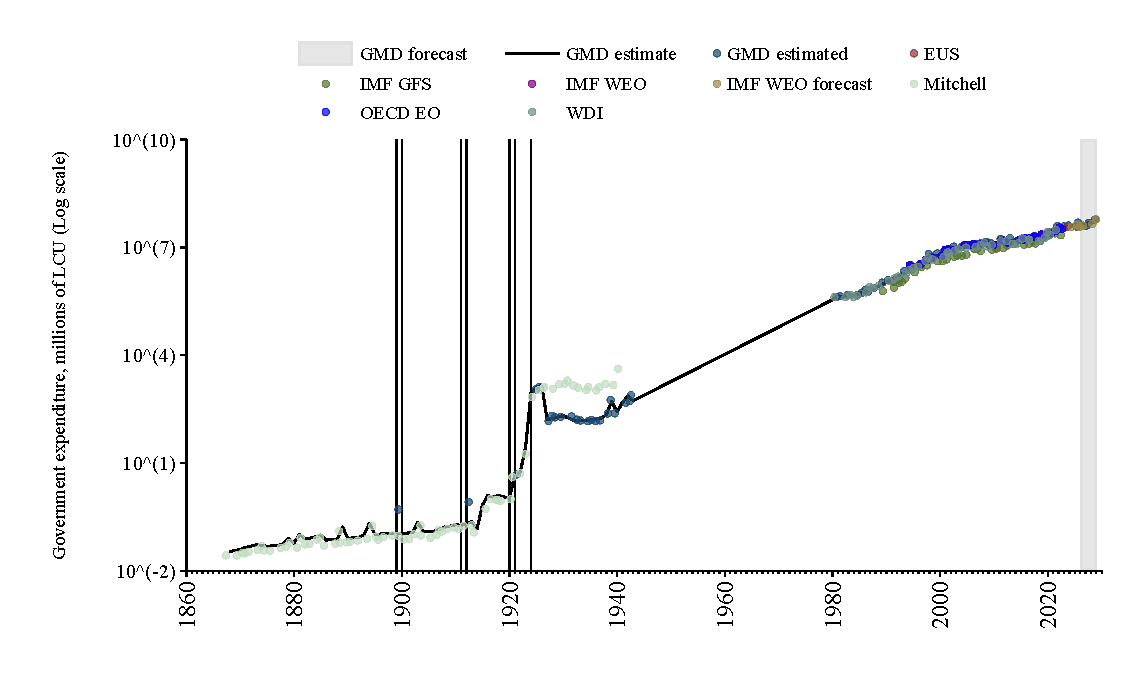
\includegraphics[width=\textwidth,height=0.6\textheight,keepaspectratio]{graphs/HUN_govexp.pdf}
\end{figure}
\end{minipage}
\end{adjustbox}
\begin{adjustbox}{max totalsize={\paperwidth}{\paperheight},center}
\begin{minipage}[t][\textheight][t]{\textwidth}
\vspace*{0.5cm}
\phantomsection
\addcontentsline{toc}{section}{Government expenditure to GDP ratio}
\begin{center}
{\Large\bfseries Government expenditure to GDP ratio}
\end{center}
\vspace{0.5cm}
\begin{table}[H]
\centering
\small
\begin{tabular}{|l|l|l|}
\hline
\textbf{Source} & \textbf{Time span} & \textbf{Notes} \\
\hline
\rowcolor{white}\cite{Mitchell}& 1900 - 1926 &Spliced using overlapping data in 1927. Data refers to central government.\\
\rowcolor{lightgray}\cite{IMF_FPP}& 1927 - 1943 &Spliced using overlapping data in 1944. Data refers to general government.\\
\rowcolor{white}\cite{WDI}& 1944 - 1994 &Spliced using overlapping data in 1995. Data refers to general government.\\
\rowcolor{lightgray}\cite{EUS}& 1995 - 2024 &Baseline source, overlaps with base year 2018. Data refers to general government.\\
\rowcolor{white}\cite{IMF_WEO_forecast}& 2025 - 2029 &Spliced using overlapping data in 2030. \\
\hline
\end{tabular}
\end{table}
\begin{figure}[H]
\centering
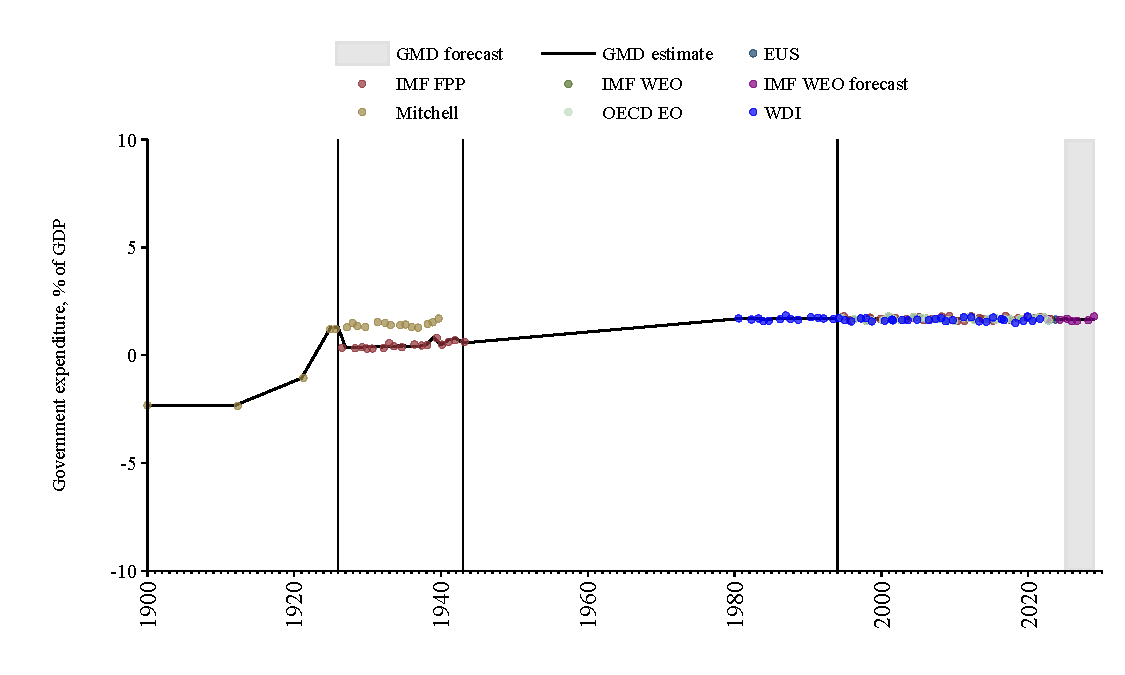
\includegraphics[width=\textwidth,height=0.6\textheight,keepaspectratio]{graphs/HUN_govexp_GDP.pdf}
\end{figure}
\end{minipage}
\end{adjustbox}
\begin{adjustbox}{max totalsize={\paperwidth}{\paperheight},center}
\begin{minipage}[t][\textheight][t]{\textwidth}
\vspace*{0.5cm}
\phantomsection
\addcontentsline{toc}{section}{Government revenue}
\begin{center}
{\Large\bfseries Government revenue}
\end{center}
\vspace{0.5cm}
\begin{table}[H]
\centering
\small
\begin{tabular}{|l|l|l|}
\hline
\textbf{Source} & \textbf{Time span} & \textbf{Notes} \\
\hline
\rowcolor{white}\cite{Mitchell}& 1868 - 1899 &Spliced using overlapping data in 1900: (ratio = 60.8\%). \\
\rowcolor{lightgray}\cite{GMD_estimated}& 1900 - 1900 &Spliced using overlapping data in 1901: (ratio = 10.3\%). \\
\rowcolor{white}\cite{Mitchell}& 1901 - 1911 &Spliced using overlapping data in 1912: (ratio = 60.8\%). \\
\rowcolor{lightgray}\cite{GMD_estimated}& 1912 - 1912 &Spliced using overlapping data in 1913: (ratio = 11.2\%). \\
\rowcolor{white}\cite{Mitchell}& 1913 - 1918 &Spliced using overlapping data in 1919: (ratio = 60.8\%). \\
\rowcolor{lightgray}\cite{GMD_estimated}& 1919 - 1921 &Spliced using overlapping data in 1922: (ratio = 78\%). \\
\rowcolor{white}\cite{Mitchell}& 1922 - 1924 &Spliced using overlapping data in 1925. \\
\rowcolor{lightgray}\cite{GMD_estimated}& 1925 - 2029 &Baseline source, overlaps with base year 2018. \\
\hline
\end{tabular}
\end{table}
\begin{figure}[H]
\centering
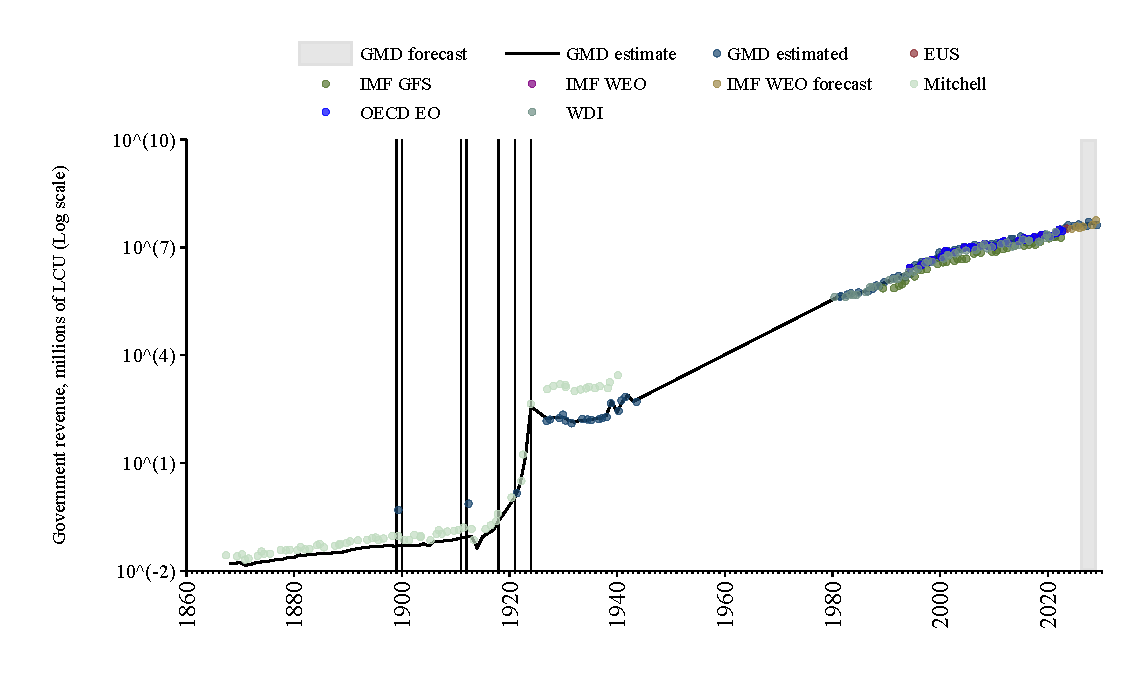
\includegraphics[width=\textwidth,height=0.6\textheight,keepaspectratio]{graphs/HUN_govrev.pdf}
\end{figure}
\end{minipage}
\end{adjustbox}
\begin{adjustbox}{max totalsize={\paperwidth}{\paperheight},center}
\begin{minipage}[t][\textheight][t]{\textwidth}
\vspace*{0.5cm}
\phantomsection
\addcontentsline{toc}{section}{Government revenue to GDP ratio}
\begin{center}
{\Large\bfseries Government revenue to GDP ratio}
\end{center}
\vspace{0.5cm}
\begin{table}[H]
\centering
\small
\begin{tabular}{|l|l|l|}
\hline
\textbf{Source} & \textbf{Time span} & \textbf{Notes} \\
\hline
\rowcolor{white}\cite{Mitchell}& 1900 - 1921 &Spliced using overlapping data in 1922. Data refers to central government.\\
\rowcolor{lightgray}\cite{IMF_FPP}& 1922 - 1943 &Spliced using overlapping data in 1944. Data refers to general government.\\
\rowcolor{white}\cite{WDI}& 1944 - 1994 &Spliced using overlapping data in 1995. Data refers to general government.\\
\rowcolor{lightgray}\cite{OECD_EO}& 1995 - 2023 &Baseline source, overlaps with base year 2018. Data refers to general government.\\
\rowcolor{white}\cite{EUS}& 2024 - 2024 &Spliced using overlapping data in 2025. Data refers to general government.\\
\rowcolor{lightgray}\cite{IMF_WEO_forecast}& 2025 - 2029 &Spliced using overlapping data in 2030. \\
\hline
\end{tabular}
\end{table}
\begin{figure}[H]
\centering
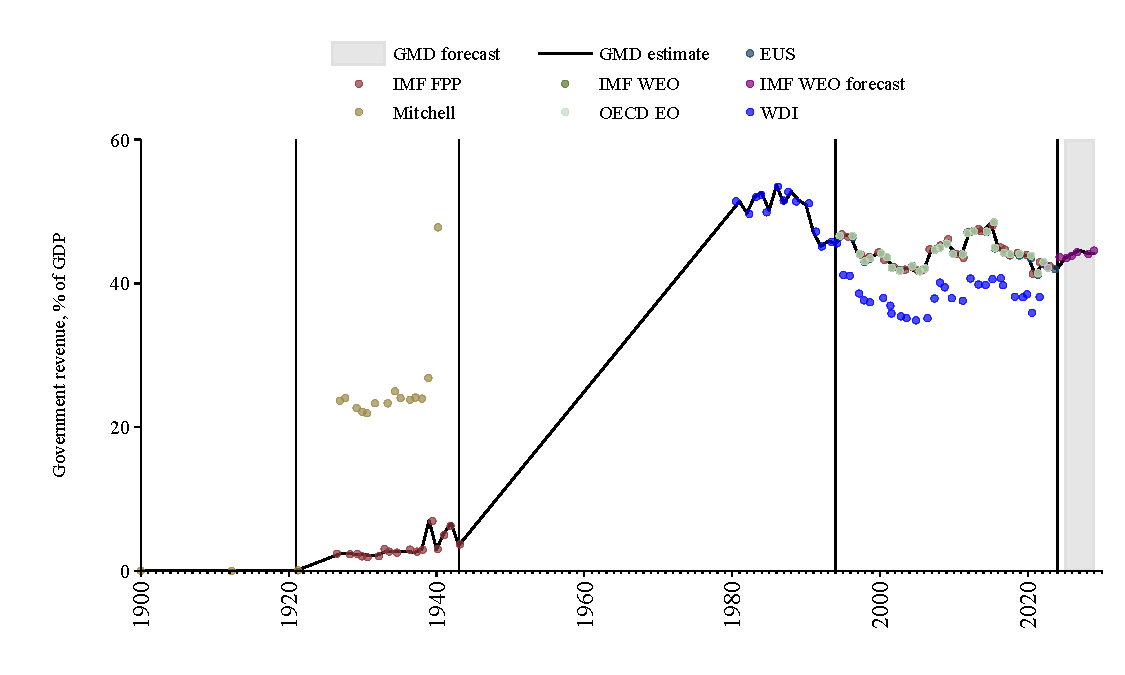
\includegraphics[width=\textwidth,height=0.6\textheight,keepaspectratio]{graphs/HUN_govrev_GDP.pdf}
\end{figure}
\end{minipage}
\end{adjustbox}
\begin{adjustbox}{max totalsize={\paperwidth}{\paperheight},center}
\begin{minipage}[t][\textheight][t]{\textwidth}
\vspace*{0.5cm}
\phantomsection
\addcontentsline{toc}{section}{Government tax revenue}
\begin{center}
{\Large\bfseries Government tax revenue}
\end{center}
\vspace{0.5cm}
\begin{table}[H]
\centering
\small
\begin{tabular}{|l|l|l|}
\hline
\textbf{Source} & \textbf{Time span} & \textbf{Notes} \\
\hline
\rowcolor{white}\cite{Mitchell}& 1868 - 1899 &Spliced using overlapping data in 1900. \\
\rowcolor{lightgray}\cite{GMD_estimated}& 1900 - 1900 &Spliced using overlapping data in 1901: (ratio = 16.9\%). \\
\rowcolor{white}\cite{Mitchell}& 1901 - 1911 &Spliced using overlapping data in 1912. \\
\rowcolor{lightgray}\cite{GMD_estimated}& 1912 - 1912 &Spliced using overlapping data in 1913: (ratio = 18.4\%). \\
\rowcolor{white}\cite{Mitchell}& 1913 - 1918 &Spliced using overlapping data in 1919. \\
\rowcolor{lightgray}\cite{GMD_estimated}& 1919 - 1921 &Spliced using overlapping data in 1922. \\
\rowcolor{white}\cite{Mitchell}& 1922 - 1924 &Spliced using overlapping data in 1925: (ratio = 128.3\%). \\
\rowcolor{lightgray}\cite{GMD_estimated}& 1925 - 2023 &Baseline source, overlaps with base year 2018. \\
\hline
\end{tabular}
\end{table}
\begin{figure}[H]
\centering
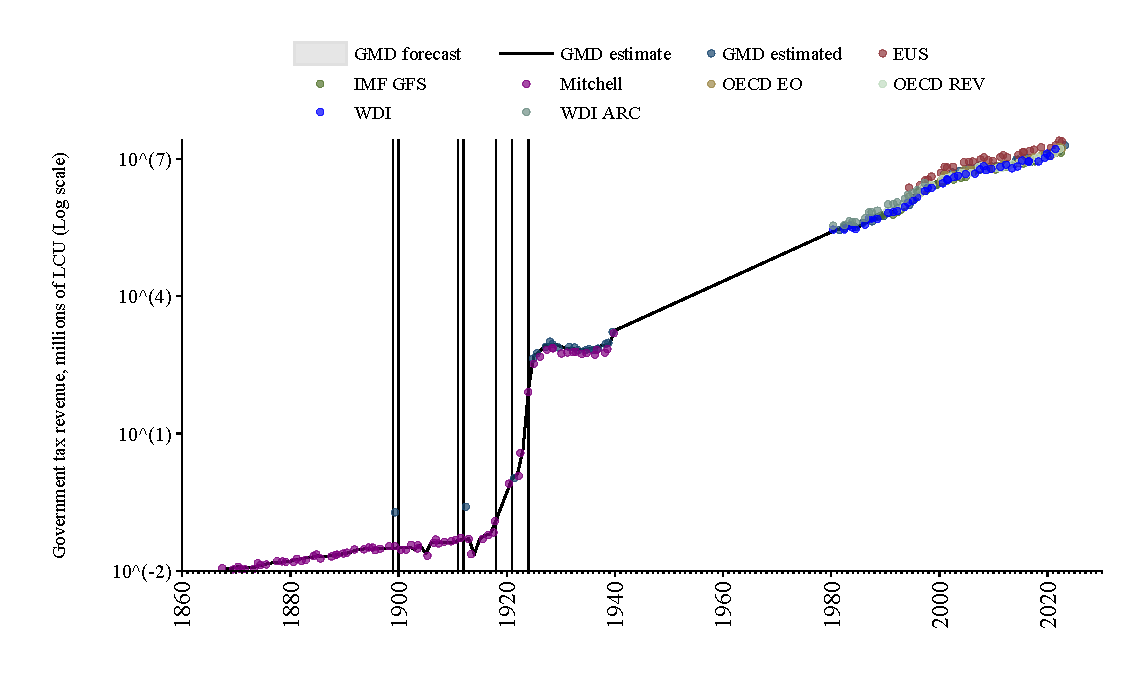
\includegraphics[width=\textwidth,height=0.6\textheight,keepaspectratio]{graphs/HUN_govtax.pdf}
\end{figure}
\end{minipage}
\end{adjustbox}
\begin{adjustbox}{max totalsize={\paperwidth}{\paperheight},center}
\begin{minipage}[t][\textheight][t]{\textwidth}
\vspace*{0.5cm}
\phantomsection
\addcontentsline{toc}{section}{Government tax revenue to GDP ratio}
\begin{center}
{\Large\bfseries Government tax revenue to GDP ratio}
\end{center}
\vspace{0.5cm}
\begin{table}[H]
\centering
\small
\begin{tabular}{|l|l|l|}
\hline
\textbf{Source} & \textbf{Time span} & \textbf{Notes} \\
\hline
\rowcolor{white}\cite{Mitchell}& 1900 - 1940 &Spliced using overlapping data in 1941. Data refers to central government.\\
\rowcolor{lightgray}\cite{WDI}& 1941 - 1994 &Spliced using overlapping data in 1995. Data refers to central government.\\
\rowcolor{white}\cite{OECD_EO}& 1995 - 2023 &Baseline source, overlaps with base year 2018. Data refers to general government.\\
\hline
\end{tabular}
\end{table}
\begin{figure}[H]
\centering
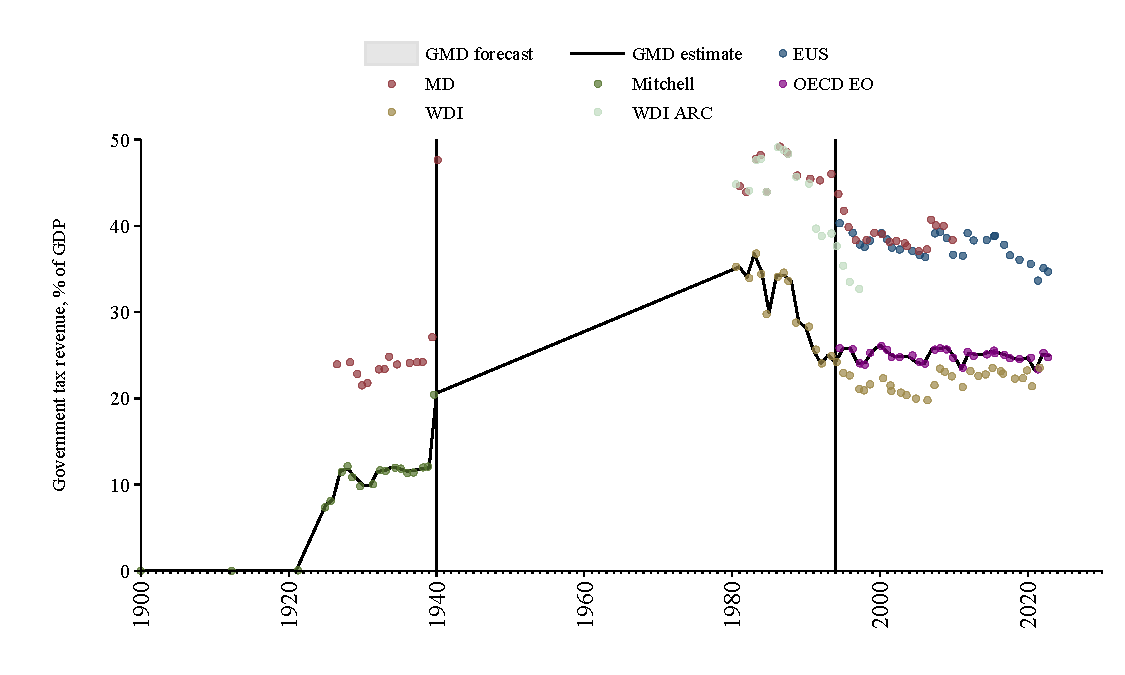
\includegraphics[width=\textwidth,height=0.6\textheight,keepaspectratio]{graphs/HUN_govtax_GDP.pdf}
\end{figure}
\end{minipage}
\end{adjustbox}
\begin{adjustbox}{max totalsize={\paperwidth}{\paperheight},center}
\begin{minipage}[t][\textheight][t]{\textwidth}
\vspace*{0.5cm}
\phantomsection
\addcontentsline{toc}{section}{Imports}
\begin{center}
{\Large\bfseries Imports}
\end{center}
\vspace{0.5cm}
\begin{table}[H]
\centering
\small
\begin{tabular}{|l|l|l|}
\hline
\textbf{Source} & \textbf{Time span} & \textbf{Notes} \\
\hline
\rowcolor{white}\cite{Tena}& 1920 - 1938 &Spliced using overlapping data in 1939: (ratio = 343.2\%). \\
\rowcolor{lightgray}\cite{Mitchell}& 1939 - 1969 &Spliced using overlapping data in 1970: (ratio = 337.9\%). \\
\rowcolor{white}\cite{UN}& 1970 - 1977 &Spliced using overlapping data in 1978: (ratio = 107.1\%). \\
\rowcolor{lightgray}\cite{AMECO}& 1978 - 1990 &Spliced using overlapping data in 1991. \\
\rowcolor{white}\cite{OECD_EO}& 1991 - 2025 &Baseline source, overlaps with base year 2018. \\
\rowcolor{lightgray}\cite{AMECO}& 2026 - 2026 &Spliced using overlapping data in 2027: (ratio = 102.4\%). \\
\rowcolor{white}\cite{IMF_WEO_forecast}& 2027 - 2029 &Spliced using overlapping data in 2030: (ratio = 104.1\%). \\
\hline
\end{tabular}
\end{table}
\begin{figure}[H]
\centering
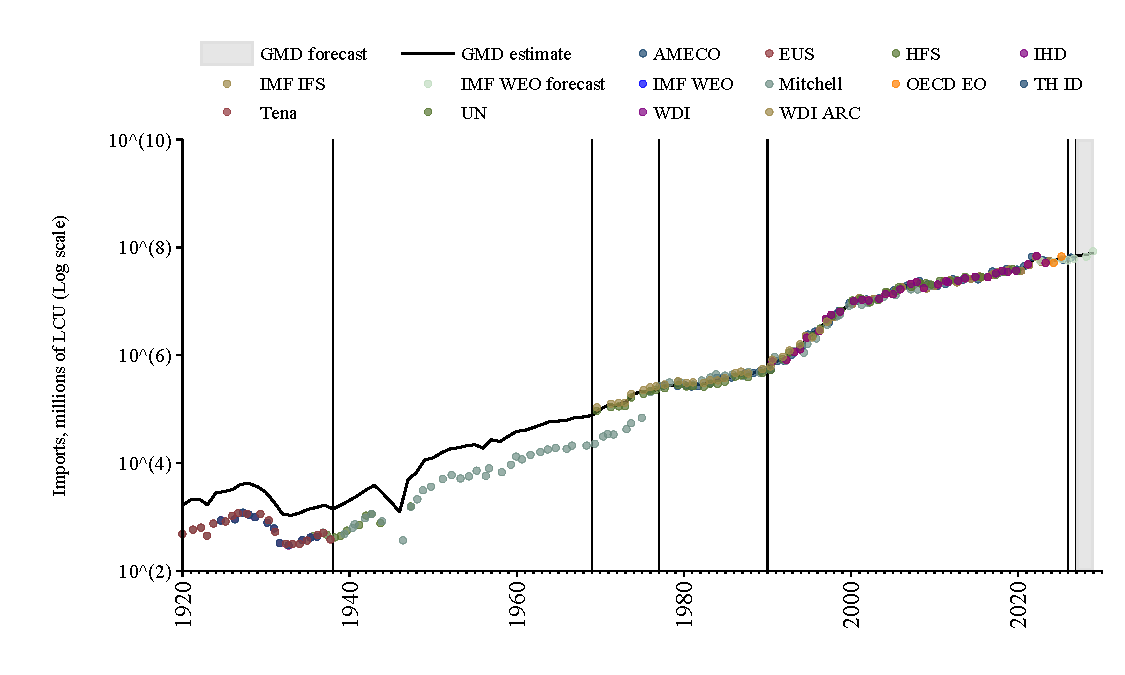
\includegraphics[width=\textwidth,height=0.6\textheight,keepaspectratio]{graphs/HUN_imports.pdf}
\end{figure}
\end{minipage}
\end{adjustbox}
\begin{adjustbox}{max totalsize={\paperwidth}{\paperheight},center}
\begin{minipage}[t][\textheight][t]{\textwidth}
\vspace*{0.5cm}
\phantomsection
\addcontentsline{toc}{section}{Imports to GDP ratio}
\begin{center}
{\Large\bfseries Imports to GDP ratio}
\end{center}
\vspace{0.5cm}
\begin{table}[H]
\centering
\small
\begin{tabular}{|l|l|l|}
\hline
\textbf{Source} & \textbf{Time span} & \textbf{Notes} \\
\hline
\rowcolor{white}\cite{Mitchell}& 1921 - 1969 &Spliced using overlapping data in 1970: (ratio = 224\%). \\
\rowcolor{lightgray}\cite{UN}& 1970 - 1990 &Spliced using overlapping data in 1991. \\
\rowcolor{white}\cite{OECD_EO}& 1991 - 2025 &Baseline source, overlaps with base year 2018. \\
\rowcolor{lightgray}\cite{AMECO}& 2026 - 2026 &Spliced using overlapping data in 2027: (ratio = 100.4\%). \\
\rowcolor{white}\cite{IMF_WEO_forecast}& 2027 - 2029 &Spliced using overlapping data in 2030: (ratio = 101\%). \\
\hline
\end{tabular}
\end{table}
\begin{figure}[H]
\centering
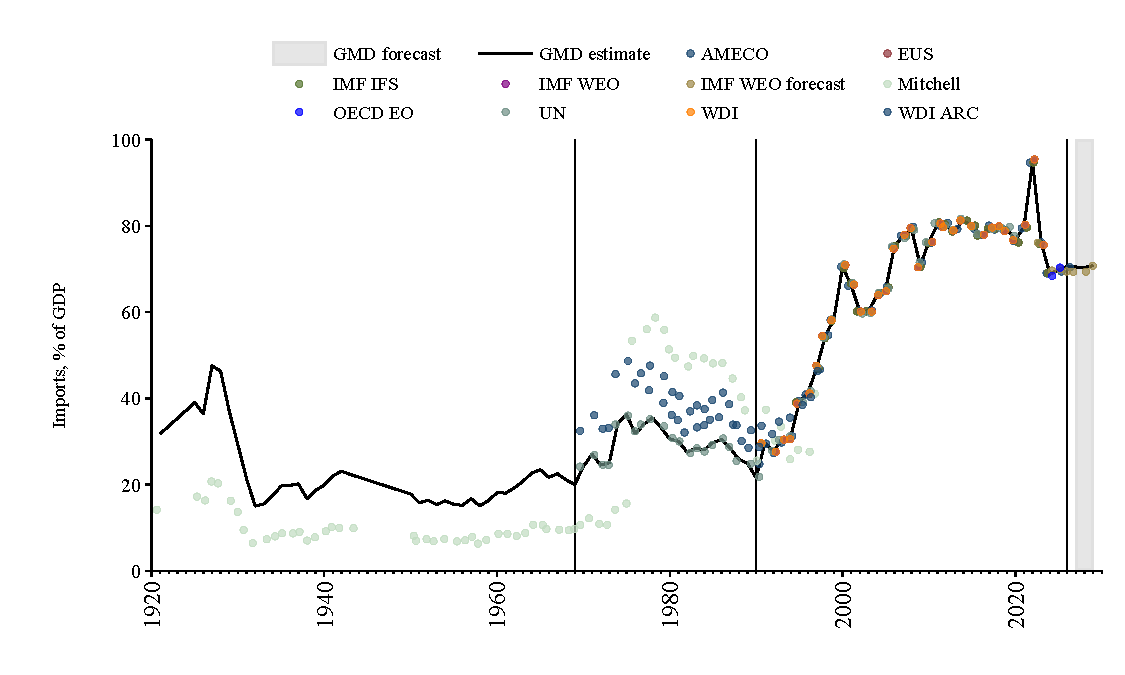
\includegraphics[width=\textwidth,height=0.6\textheight,keepaspectratio]{graphs/HUN_imports_GDP.pdf}
\end{figure}
\end{minipage}
\end{adjustbox}
\begin{adjustbox}{max totalsize={\paperwidth}{\paperheight},center}
\begin{minipage}[t][\textheight][t]{\textwidth}
\vspace*{0.5cm}
\phantomsection
\addcontentsline{toc}{section}{Inflation}
\begin{center}
{\Large\bfseries Inflation}
\end{center}
\vspace{0.5cm}
\begin{table}[H]
\centering
\small
\begin{tabular}{|l|l|l|}
\hline
\textbf{Source} & \textbf{Time span} & \textbf{Notes} \\
\hline
\rowcolor{white}\cite{RR}& 1924 - 1924 &Spliced using overlapping data in 1925. \\
\rowcolor{lightgray}\cite{CLIO}& 1925 - 1928 &Spliced using overlapping data in 1929. \\
\rowcolor{white}\cite{RR}& 1929 - 1929 &Spliced using overlapping data in 1930. \\
\rowcolor{lightgray}\cite{CLIO}& 1930 - 1934 &Spliced using overlapping data in 1935. \\
\rowcolor{white}\cite{RR}& 1935 - 1935 &Spliced using overlapping data in 1936. \\
\rowcolor{lightgray}\cite{CLIO}& 1936 - 1945 &Spliced using overlapping data in 1946. \\
\rowcolor{white}\cite{RR}& 1946 - 1946 &Spliced using overlapping data in 1947. \\
\rowcolor{lightgray}\cite{CLIO}& 1947 - 1952 &Spliced using overlapping data in 1953. \\
\rowcolor{white}\cite{RR}& 1953 - 1953 &Spliced using overlapping data in 1954. \\
\rowcolor{lightgray}\cite{CLIO}& 1954 - 1957 &Spliced using overlapping data in 1958. \\
\rowcolor{white}\cite{RR}& 1958 - 1958 &Spliced using overlapping data in 1959. \\
\rowcolor{lightgray}\cite{CLIO}& 1959 - 1959 &Spliced using overlapping data in 1960. \\
\rowcolor{white}\cite{RR}& 1960 - 1961 &Spliced using overlapping data in 1962. \\
\rowcolor{lightgray}\cite{CLIO}& 1962 - 1965 &Spliced using overlapping data in 1966. \\
\rowcolor{white}\cite{RR}& 1966 - 1966 &Spliced using overlapping data in 1967. \\
\rowcolor{lightgray}\cite{CLIO}& 1967 - 1967 &Spliced using overlapping data in 1968. \\
\rowcolor{white}\cite{RR}& 1968 - 1968 &Spliced using overlapping data in 1969. \\
\rowcolor{lightgray}\cite{CLIO}& 1969 - 1969 &Spliced using overlapping data in 1970. \\
\rowcolor{white}\cite{WB_CC}& 1970 - 2023 &Baseline source, overlaps with base year 2018. \\
\rowcolor{lightgray}\cite{BIS}& 2024 - 2024 &Spliced using overlapping data in 2025. \\
\rowcolor{white}\cite{IMF_WEO_forecast}& 2025 - 2029 &Spliced using overlapping data in 2030. \\
\hline
\end{tabular}
\end{table}
\begin{figure}[H]
\centering
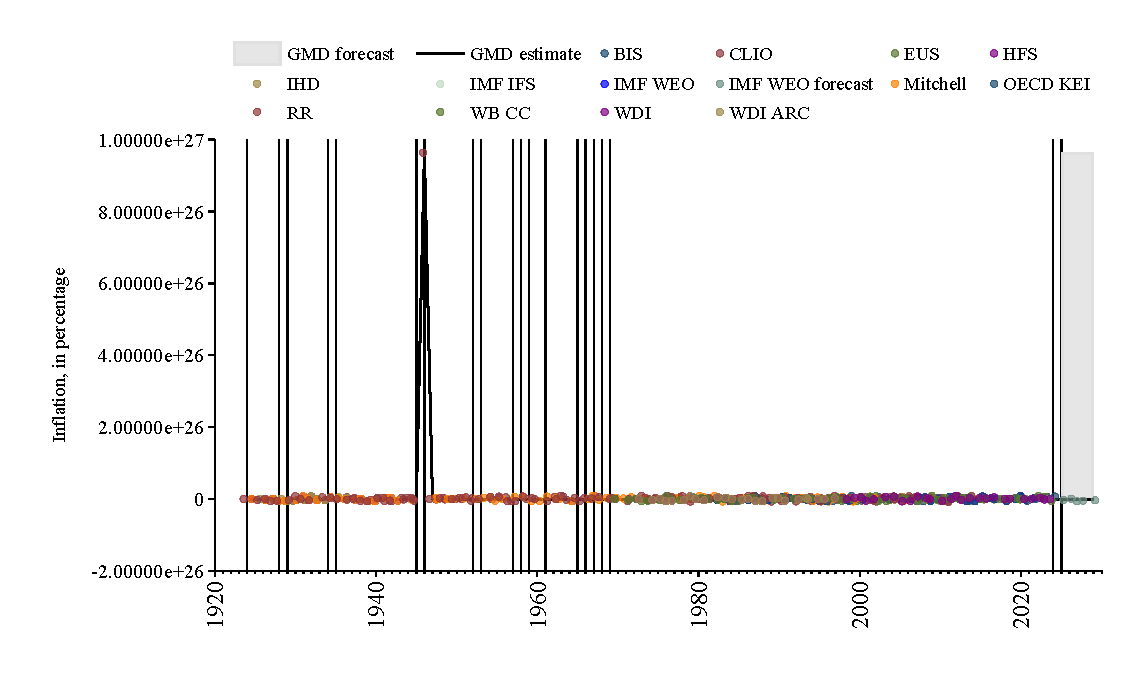
\includegraphics[width=\textwidth,height=0.6\textheight,keepaspectratio]{graphs/HUN_infl.pdf}
\end{figure}
\end{minipage}
\end{adjustbox}
\begin{adjustbox}{max totalsize={\paperwidth}{\paperheight},center}
\begin{minipage}[t][\textheight][t]{\textwidth}
\vspace*{0.5cm}
\phantomsection
\addcontentsline{toc}{section}{Investment}
\begin{center}
{\Large\bfseries Investment}
\end{center}
\vspace{0.5cm}
\begin{table}[H]
\centering
\small
\begin{tabular}{|l|l|l|}
\hline
\textbf{Source} & \textbf{Time span} & \textbf{Notes} \\
\hline
\rowcolor{white}\cite{Mitchell}& 1925 - 1959 &Spliced using overlapping data in 1960: (ratio = 238.3\%). \\
\rowcolor{lightgray}\cite{WDI_ARC}& 1960 - 1969 &Spliced using overlapping data in 1970: (ratio = 118.7\%). \\
\rowcolor{white}\cite{AMECO}& 1970 - 1990 &Spliced using overlapping data in 1991: (ratio = 98.5\%). \\
\rowcolor{lightgray}\cite{OECD_EO}& 1991 - 2025 &Baseline source, overlaps with base year 2018. \\
\rowcolor{white}\cite{AMECO}& 2026 - 2026 &Spliced using overlapping data in 2027: (ratio = 115.3\%). \\
\rowcolor{lightgray}\cite{IMF_WEO_forecast}& 2027 - 2029 &Spliced using overlapping data in 2030: (ratio = 109\%). \\
\hline
\end{tabular}
\end{table}
\begin{figure}[H]
\centering
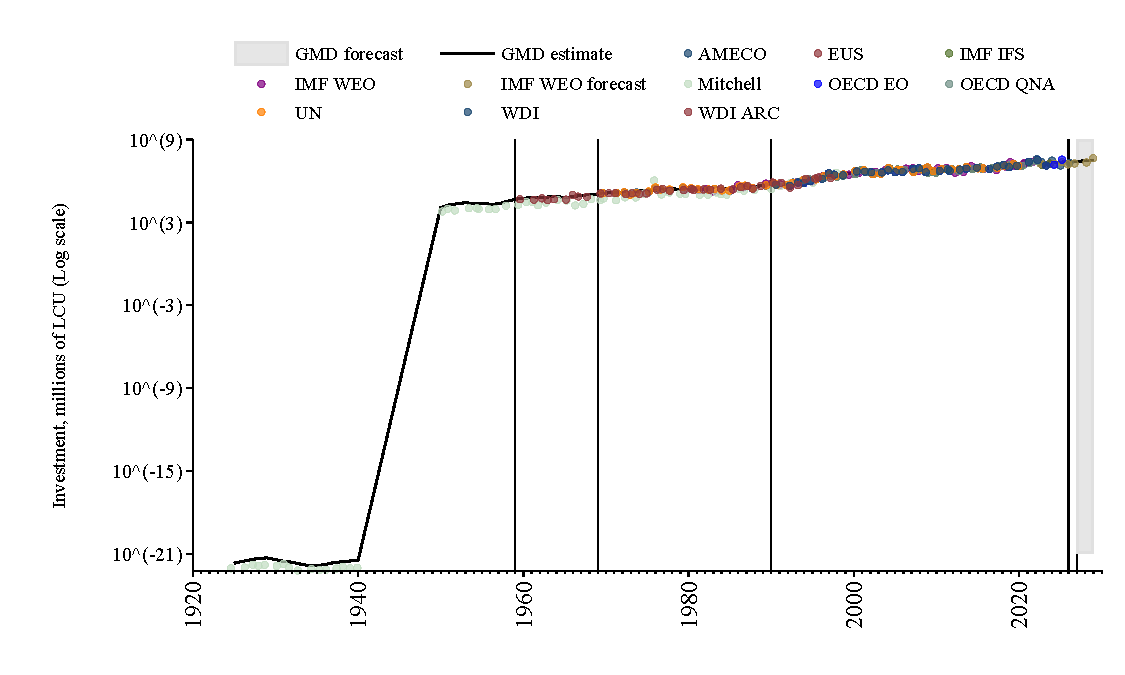
\includegraphics[width=\textwidth,height=0.6\textheight,keepaspectratio]{graphs/HUN_inv.pdf}
\end{figure}
\end{minipage}
\end{adjustbox}
\begin{adjustbox}{max totalsize={\paperwidth}{\paperheight},center}
\begin{minipage}[t][\textheight][t]{\textwidth}
\vspace*{0.5cm}
\phantomsection
\addcontentsline{toc}{section}{Investment to GDP ratio}
\begin{center}
{\Large\bfseries Investment to GDP ratio}
\end{center}
\vspace{0.5cm}
\begin{table}[H]
\centering
\small
\begin{tabular}{|l|l|l|}
\hline
\textbf{Source} & \textbf{Time span} & \textbf{Notes} \\
\hline
\rowcolor{white}\cite{Mitchell}& 1925 - 1959 &Spliced using overlapping data in 1960: (ratio = 166.7\%). \\
\rowcolor{lightgray}\cite{WDI_ARC}& 1960 - 1990 &Spliced using overlapping data in 1991: (ratio = 102.5\%). \\
\rowcolor{white}\cite{OECD_EO}& 1991 - 2025 &Baseline source, overlaps with base year 2018. \\
\rowcolor{lightgray}\cite{AMECO}& 2026 - 2026 &Spliced using overlapping data in 2027: (ratio = 113\%). \\
\rowcolor{white}\cite{IMF_WEO_forecast}& 2027 - 2029 &Spliced using overlapping data in 2030: (ratio = 105.7\%). \\
\hline
\end{tabular}
\end{table}
\begin{figure}[H]
\centering
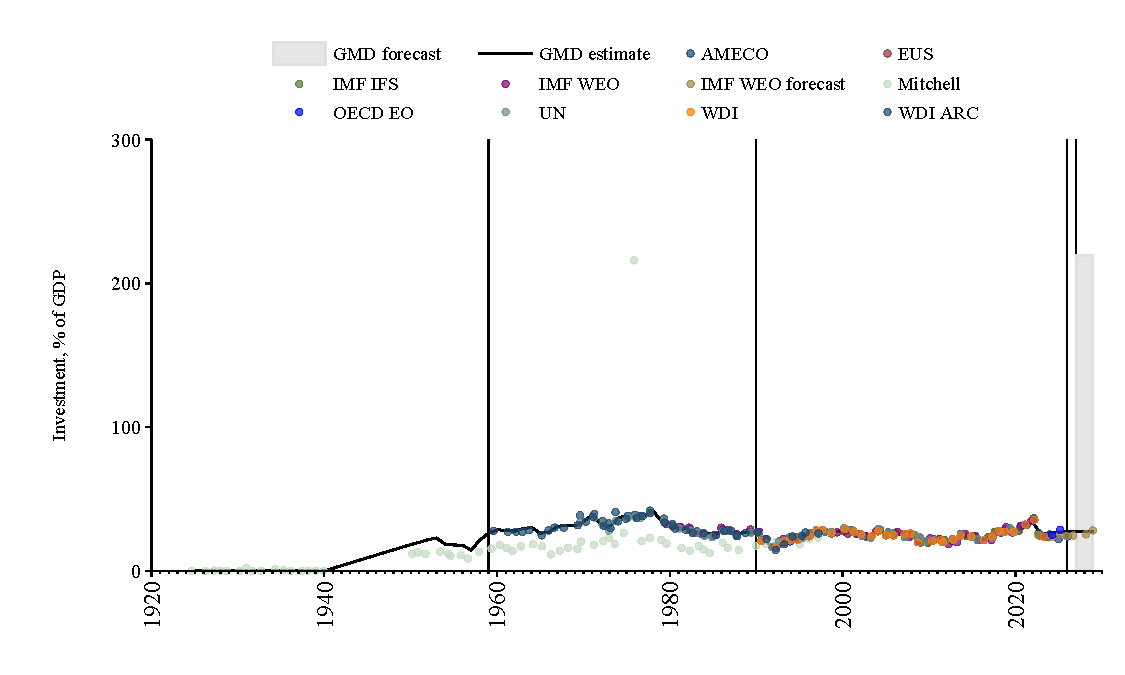
\includegraphics[width=\textwidth,height=0.6\textheight,keepaspectratio]{graphs/HUN_inv_GDP.pdf}
\end{figure}
\end{minipage}
\end{adjustbox}
\begin{adjustbox}{max totalsize={\paperwidth}{\paperheight},center}
\begin{minipage}[t][\textheight][t]{\textwidth}
\vspace*{0.5cm}
\phantomsection
\addcontentsline{toc}{section}{Long term interest rate}
\begin{center}
{\Large\bfseries Long term interest rate}
\end{center}
\vspace{0.5cm}
\begin{table}[H]
\centering
\small
\begin{tabular}{|l|l|l|}
\hline
\textbf{Source} & \textbf{Time span} & \textbf{Notes} \\
\hline
\rowcolor{white}\cite{AMECO}& 1999 - 1999 &Spliced using overlapping data in 2000. \\
\rowcolor{lightgray}\cite{OECD_MEI}& 2000 - 2023 &Baseline source, overlaps with base year 2018. \\
\rowcolor{white}\cite{EUS}& 2024 - 2024 &Spliced using overlapping data in 2025. \\
\hline
\end{tabular}
\end{table}
\begin{figure}[H]
\centering
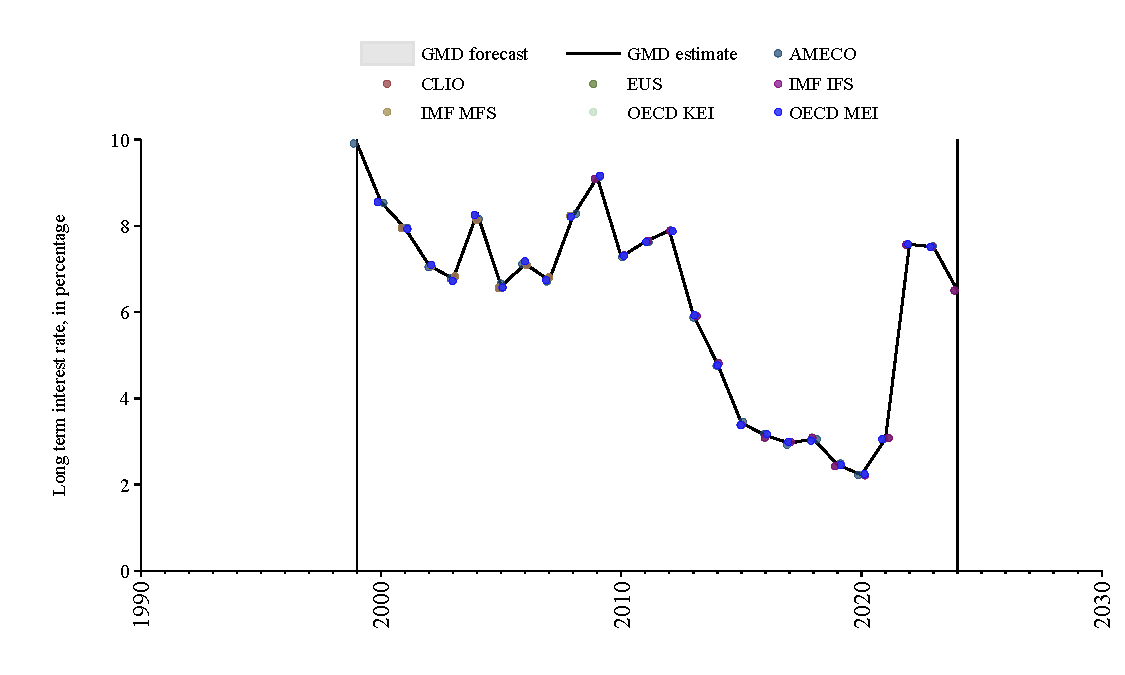
\includegraphics[width=\textwidth,height=0.6\textheight,keepaspectratio]{graphs/HUN_ltrate.pdf}
\end{figure}
\end{minipage}
\end{adjustbox}
\begin{adjustbox}{max totalsize={\paperwidth}{\paperheight},center}
\begin{minipage}[t][\textheight][t]{\textwidth}
\vspace*{0.5cm}
\phantomsection
\addcontentsline{toc}{section}{Nominal GDP}
\begin{center}
{\Large\bfseries Nominal GDP}
\end{center}
\vspace{0.5cm}
\begin{table}[H]
\centering
\small
\begin{tabular}{|l|l|l|}
\hline
\textbf{Source} & \textbf{Time span} & \textbf{Notes} \\
\hline
\rowcolor{white}\cite{NBS}& 1870 - 1899 &Spliced using overlapping data in 1900: (ratio = 164.6\%). \\
\rowcolor{lightgray}\cite{Mitchell}& 1900 - 1900 &Spliced using overlapping data in 1901: (ratio = 590.2\%). \\
\rowcolor{white}\cite{NBS}& 1901 - 1911 &Spliced using overlapping data in 1912: (ratio = 164.6\%). \\
\rowcolor{lightgray}\cite{Mitchell}& 1912 - 1912 &Spliced using overlapping data in 1913: (ratio = 543.6\%). \\
\rowcolor{white}\cite{NBS}& 1913 - 1913 &Spliced using overlapping data in 1914: (ratio = 164.6\%). \\
\rowcolor{lightgray}\cite{Mitchell}& 1914 - 1959 &Spliced using overlapping data in 1960: (ratio = 128.3\%). \\
\rowcolor{white}\cite{WDI}& 1960 - 1969 &Spliced using overlapping data in 1970. \\
\rowcolor{lightgray}\cite{AMECO}& 1970 - 1990 &Spliced using overlapping data in 1991: (ratio = 99.7\%). \\
\rowcolor{white}\cite{OECD_EO}& 1991 - 2025 &Baseline source, overlaps with base year 2018. \\
\rowcolor{lightgray}\cite{AMECO}& 2026 - 2026 &Spliced using overlapping data in 2027: (ratio = 102\%). \\
\rowcolor{white}\cite{IMF_WEO_forecast}& 2027 - 2029 &Spliced using overlapping data in 2030: (ratio = 103.1\%). \\
\hline
\end{tabular}
\end{table}
\begin{figure}[H]
\centering
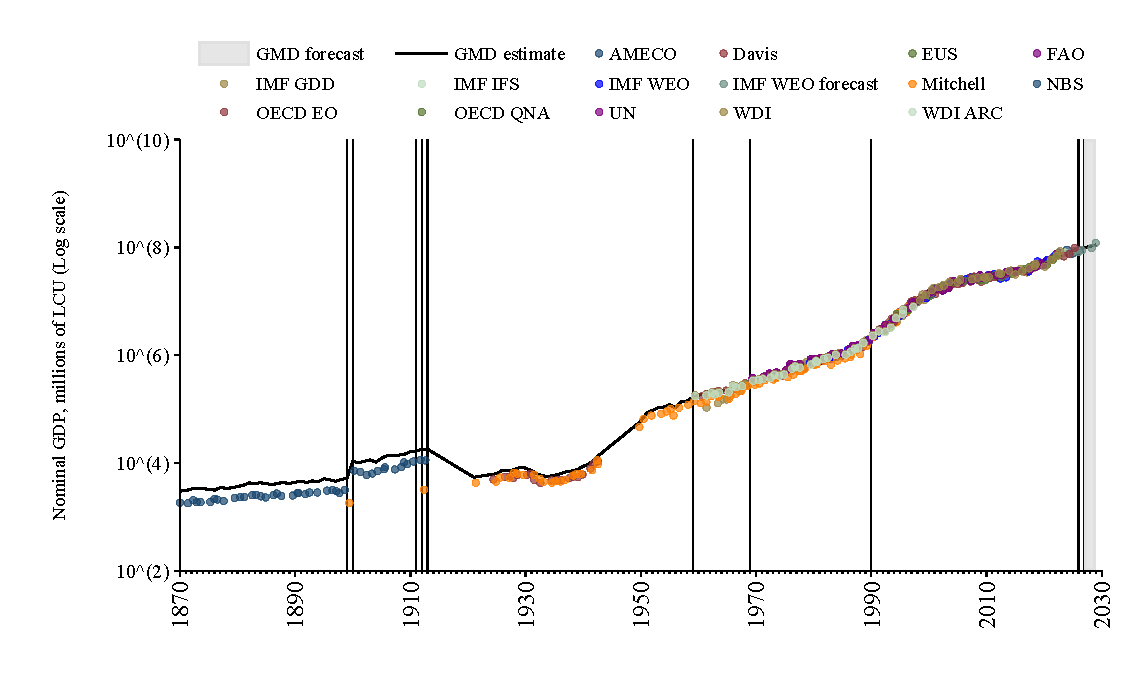
\includegraphics[width=\textwidth,height=0.6\textheight,keepaspectratio]{graphs/HUN_nGDP.pdf}
\end{figure}
\end{minipage}
\end{adjustbox}
\begin{adjustbox}{max totalsize={\paperwidth}{\paperheight},center}
\begin{minipage}[t][\textheight][t]{\textwidth}
\vspace*{0.5cm}
\phantomsection
\addcontentsline{toc}{section}{Population}
\begin{center}
{\Large\bfseries Population}
\end{center}
\vspace{0.5cm}
\begin{table}[H]
\centering
\small
\begin{tabular}{|l|l|l|}
\hline
\textbf{Source} & \textbf{Time span} & \textbf{Notes} \\
\hline
\rowcolor{white}\cite{Gapminder}& 1800 - 1949 &Spliced using overlapping data in 1950: (ratio = 99.8\%). \\
\rowcolor{lightgray}\cite{IMF_IFS}& 1950 - 1959 &Spliced using overlapping data in 1960: (ratio = 99.8\%). \\
\rowcolor{white}\cite{WDI}& 1960 - 2023 &Baseline source, overlaps with base year 2018. \\
\rowcolor{lightgray}\cite{OECD_EO}& 2024 - 2025 &Spliced using overlapping data in 2026: (ratio = 99.4\%). \\
\rowcolor{white}\cite{AMECO}& 2026 - 2026 &Spliced using overlapping data in 2027: (ratio = 100.1\%). \\
\rowcolor{lightgray}\cite{Gapminder}& 2027 - 2030 &Spliced using overlapping data in 2031: (ratio = 99.4\%). \\
\hline
\end{tabular}
\end{table}
\begin{figure}[H]
\centering
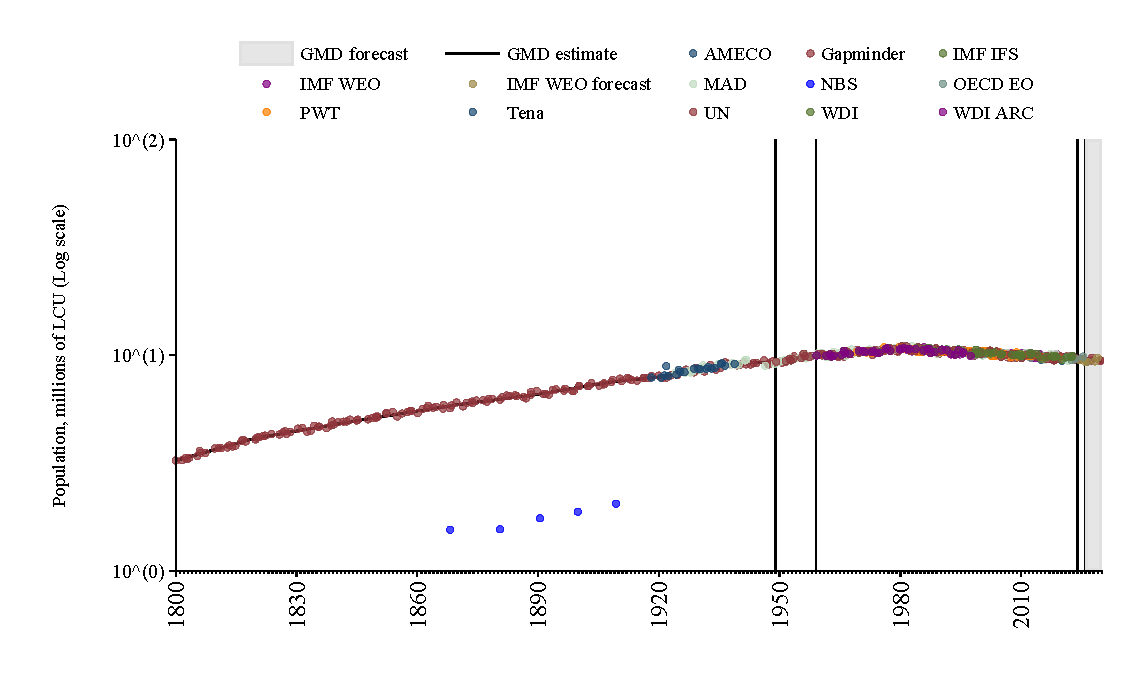
\includegraphics[width=\textwidth,height=0.6\textheight,keepaspectratio]{graphs/HUN_pop.pdf}
\end{figure}
\end{minipage}
\end{adjustbox}
\begin{adjustbox}{max totalsize={\paperwidth}{\paperheight},center}
\begin{minipage}[t][\textheight][t]{\textwidth}
\vspace*{0.5cm}
\phantomsection
\addcontentsline{toc}{section}{Real GDP}
\begin{center}
{\Large\bfseries Real GDP}
\end{center}
\vspace{0.5cm}
\begin{table}[H]
\centering
\small
\begin{tabular}{|l|l|l|}
\hline
\textbf{Source} & \textbf{Time span} & \textbf{Notes} \\
\hline
\rowcolor{white}\cite{NBS}& 1870 - 1913 &Spliced using overlapping data in 1914: (ratio = 4.01e+08\%). \\
\rowcolor{lightgray}\cite{Mitchell}& 1914 - 1943 &Spliced using overlapping data in 1944: (ratio = 200239.2\%). \\
\rowcolor{white}\cite{MAD}& 1944 - 1949 &Spliced using overlapping data in 1950: (ratio = 4474.8\%). \\
\rowcolor{lightgray}\cite{Mitchell}& 1950 - 1959 &Spliced using overlapping data in 1960: (ratio = 3624\%). \\
\rowcolor{white}\cite{WDI}& 1960 - 1990 &Spliced using overlapping data in 1991. \\
\rowcolor{lightgray}\cite{OECD_EO}& 1991 - 2025 &Baseline source, overlaps with base year 2018. \\
\rowcolor{white}\cite{AMECO}& 2026 - 2026 &Spliced using overlapping data in 2027: (ratio = 102\%). \\
\rowcolor{lightgray}\cite{IMF_WEO_forecast}& 2027 - 2029 &Spliced using overlapping data in 2030: (ratio = 100.6\%). \\
\hline
\end{tabular}
\end{table}
\begin{figure}[H]
\centering
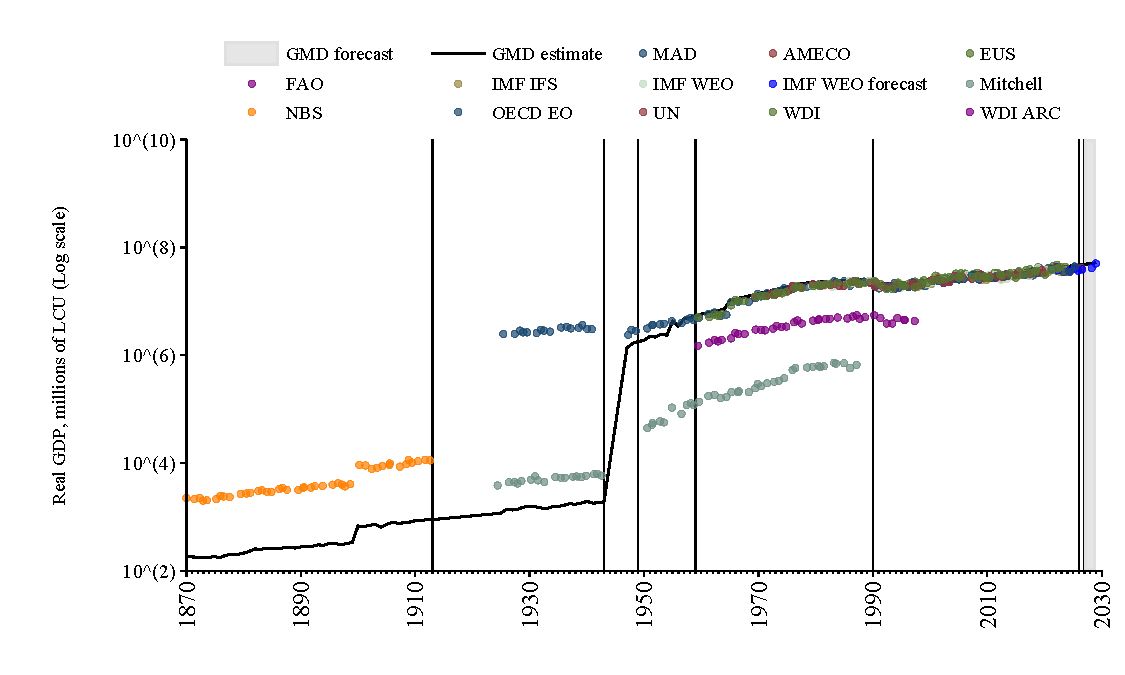
\includegraphics[width=\textwidth,height=0.6\textheight,keepaspectratio]{graphs/HUN_rGDP.pdf}
\end{figure}
\end{minipage}
\end{adjustbox}
\begin{adjustbox}{max totalsize={\paperwidth}{\paperheight},center}
\begin{minipage}[t][\textheight][t]{\textwidth}
\vspace*{0.5cm}
\phantomsection
\addcontentsline{toc}{section}{Real total consumption}
\begin{center}
{\Large\bfseries Real total consumption}
\end{center}
\vspace{0.5cm}
\begin{table}[H]
\centering
\small
\begin{tabular}{|l|l|l|}
\hline
\textbf{Source} & \textbf{Time span} & \textbf{Notes} \\
\hline
\rowcolor{white}\cite{UN}& 1970 - 1990 &Spliced using overlapping data in 1991: (ratio = 90.4\%). \\
\rowcolor{lightgray}\cite{WDI}& 1991 - 1994 &Spliced using overlapping data in 1995: (ratio = 89.6\%). \\
\rowcolor{white}\cite{IMF_IFS}& 1995 - 2024 &Baseline source, overlaps with base year 2018. \\
\hline
\end{tabular}
\end{table}
\begin{figure}[H]
\centering
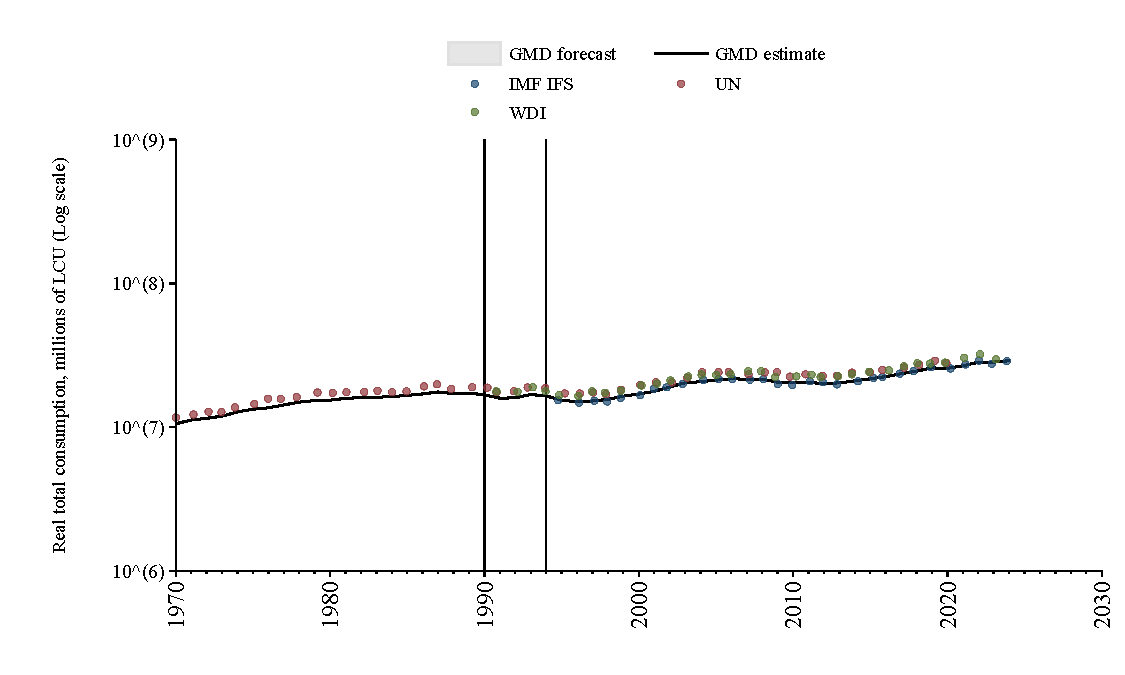
\includegraphics[width=\textwidth,height=0.6\textheight,keepaspectratio]{graphs/HUN_rcons.pdf}
\end{figure}
\end{minipage}
\end{adjustbox}
\begin{adjustbox}{max totalsize={\paperwidth}{\paperheight},center}
\begin{minipage}[t][\textheight][t]{\textwidth}
\vspace*{0.5cm}
\phantomsection
\addcontentsline{toc}{section}{Short term interest rate}
\begin{center}
{\Large\bfseries Short term interest rate}
\end{center}
\vspace{0.5cm}
\begin{table}[H]
\centering
\small
\begin{tabular}{|l|l|l|}
\hline
\textbf{Source} & \textbf{Time span} & \textbf{Notes} \\
\hline
\rowcolor{white}\cite{NBS}& 1863 - 1913 &Spliced using overlapping data in 1914. \\
\rowcolor{lightgray}\cite{IHD}& 1914 - 1936 &Spliced using overlapping data in 1937. \\
\rowcolor{white}\cite{IMF_MFS}& 1937 - 2008 &Spliced using overlapping data in 2009. \\
\rowcolor{lightgray}\cite{OECD_EO}& 2009 - 2009 &Spliced using overlapping data in 2010. \\
\rowcolor{white}\cite{OECD_KEI}& 2010 - 2011 &Spliced using overlapping data in 2012. \\
\rowcolor{lightgray}\cite{OECD_EO}& 2012 - 2013 &Spliced using overlapping data in 2014. \\
\rowcolor{white}\cite{OECD_KEI}& 2014 - 2023 &Baseline source, overlaps with base year 2018. \\
\rowcolor{lightgray}\cite{OECD_EO}& 2024 - 2025 &Spliced using overlapping data in 2026. \\
\hline
\end{tabular}
\end{table}
\begin{figure}[H]
\centering
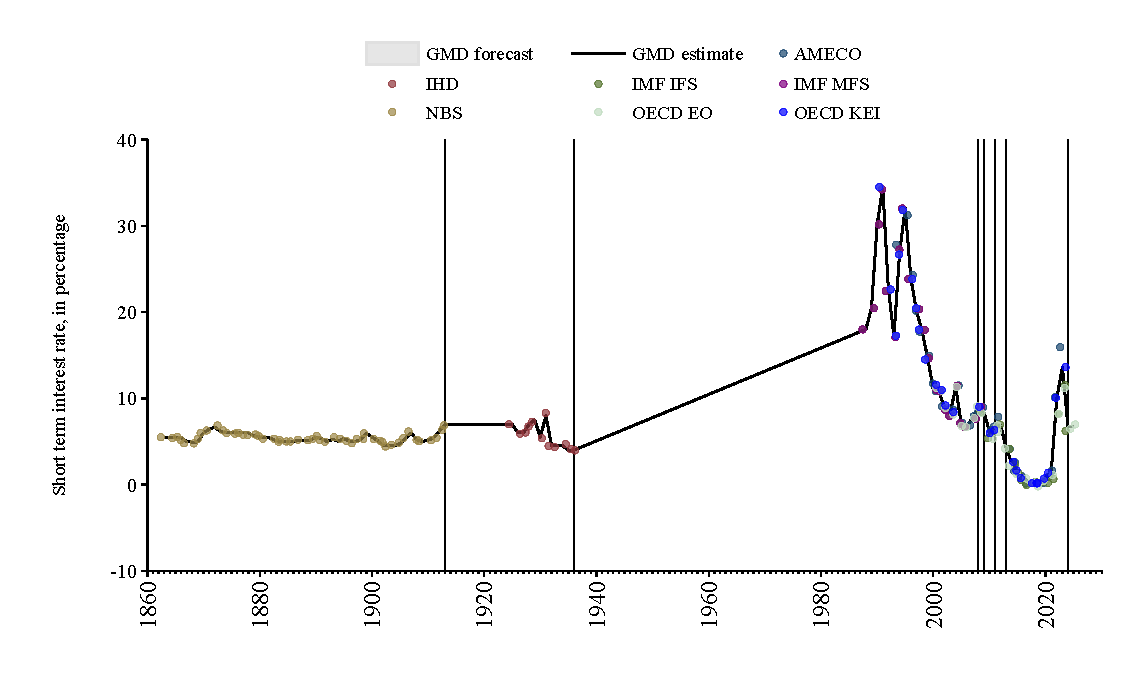
\includegraphics[width=\textwidth,height=0.6\textheight,keepaspectratio]{graphs/HUN_strate.pdf}
\end{figure}
\end{minipage}
\end{adjustbox}
\begin{adjustbox}{max totalsize={\paperwidth}{\paperheight},center}
\begin{minipage}[t][\textheight][t]{\textwidth}
\vspace*{0.5cm}
\phantomsection
\addcontentsline{toc}{section}{Unemployment}
\begin{center}
{\Large\bfseries Unemployment}
\end{center}
\vspace{0.5cm}
\begin{table}[H]
\centering
\small
\begin{tabular}{|l|l|l|}
\hline
\textbf{Source} & \textbf{Time span} & \textbf{Notes} \\
\hline
\rowcolor{white}\cite{IMF_WEO}& 1980 - 1991 &Spliced using overlapping data in 1992. \\
\rowcolor{lightgray}\cite{OECD_EO}& 1992 - 2008 &Spliced using overlapping data in 2009. \\
\rowcolor{white}\cite{EUS}& 2009 - 2024 &Baseline source, overlaps with base year 2018. \\
\rowcolor{lightgray}\cite{OECD_EO}& 2025 - 2025 &Spliced using overlapping data in 2026. \\
\rowcolor{white}\cite{AMECO}& 2026 - 2026 &Spliced using overlapping data in 2027. \\
\rowcolor{lightgray}\cite{IMF_WEO_forecast}& 2027 - 2029 &Spliced using overlapping data in 2030. \\
\hline
\end{tabular}
\end{table}
\begin{figure}[H]
\centering
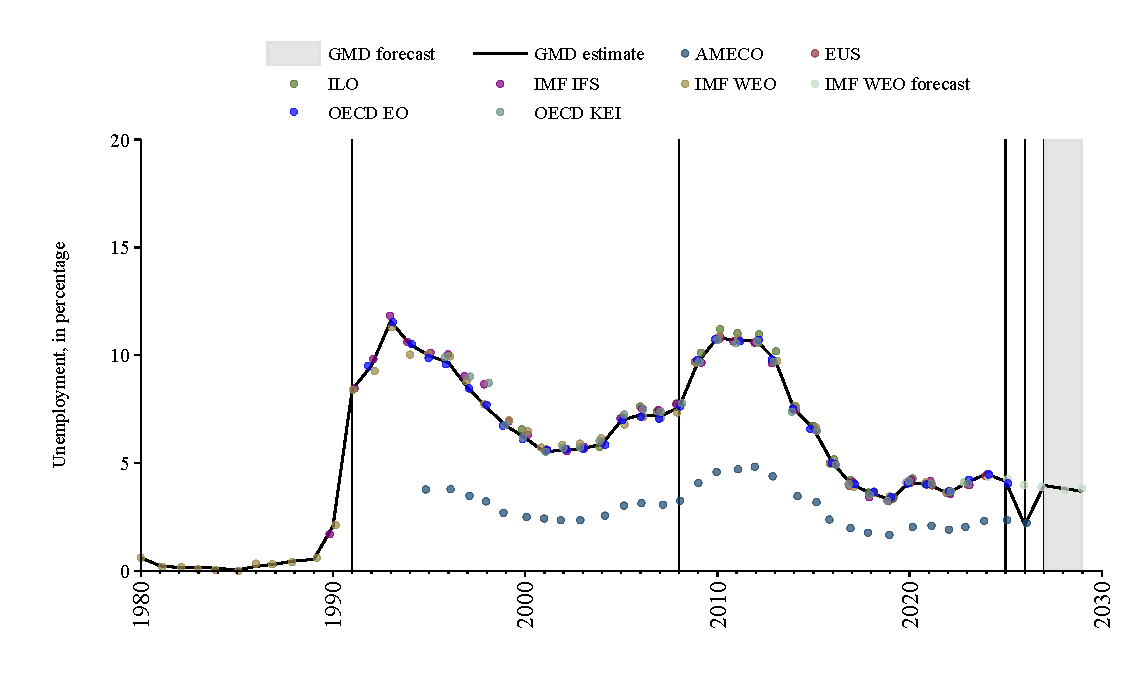
\includegraphics[width=\textwidth,height=0.6\textheight,keepaspectratio]{graphs/HUN_unemp.pdf}
\end{figure}
\end{minipage}
\end{adjustbox}
\phantomsection
\addcontentsline{toc}{section}{References}
\begin{center}
{\Large\bfseries References}
\end{center}
\small
\bibliographystyle{qje}
\bibliography{bib}
\end{document}
